\documentclass{article}

%%%%%%%%%%%%%%%%%%%%%%%%%%%%%%%%%%%%%%%% packages
\usepackage{myPackages}
\usepackage[utf8]{inputenc}
\usepackage{mathtools}
\usepackage{amssymb}
\usepackage{amsmath}
\usepackage{amsthm}
\usepackage{listings}
\usepackage[b]{esvect}
\usepackage[toc,page]{appendix}

%%%%%%%%%%%%%%%%%%%%%%%%%%%%%%%%%%%%%%%%
\DeclareMathOperator{\arctantwo}{arctan2}

%%%%%%%%%%%%%%%%%%%%%%%%%%%%%%%%%%%%%%%% title...
\title{Adaptive Cell Decomposition\\
A Space Subdivision Method Beyond Lines}
% \author{Saeed Gholami Shahbandi, Adam Duracz}
% \date{March 2016}

%%%%%%%%%%%%%%%%%%%%%%%%%%%%%%%%%%%%%%%%
\begin{document}
\maketitle

%\section{Introduction}
% what is ``Space subdivision''
Subdivision is the process of partitioning a space $\mathcal{S}$, according to a provided set of level-curves $\mathcal{C}$ in that space, into a set of faces $\mathcal{F}$.
%% \footnote{for simplicity, level-curves will be refered to as curves in the rest of the document.} 

\[ \mathit{subdivision}(\mathcal{C}): \mathcal{S} \xrightarrow[]{decompose} \mathcal{F}\left(\mathcal{C}\right) \]

Figure~\ref{fig:intro_curvesPartitioning1} shows an example of a planar subdivision (where $\mathcal{S}$ is two dimensional), according to a set of curves containing six straight lines.
% what is it useful for? some application?
The process of subdivision provides an abstraction of the space.
Such an abstraction potentially facilitates some geometric processes required on that space.

\begin{figure}%[!ht]
  \centering
  \begin{subfigure}{.4\textwidth}
    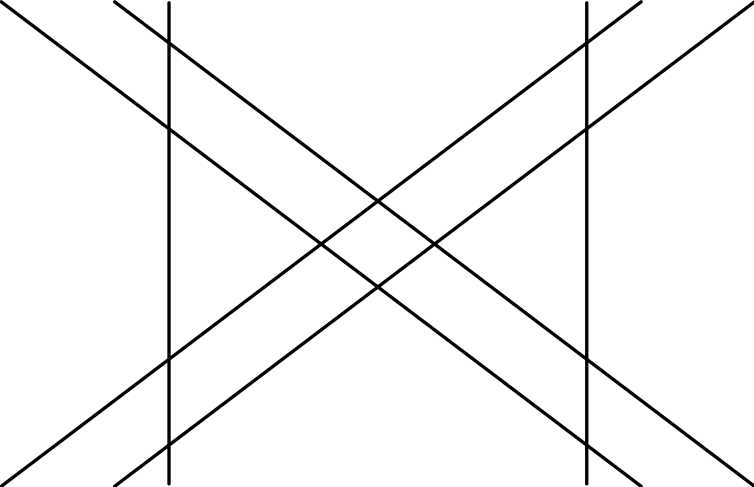
\includegraphics[width=\textwidth]{figures/intro_curves1.png}
    \caption{curves} \label{subfig:intro_curves1}
  \end{subfigure}%
  \quad \quad \quad%
  \begin{subfigure}{.4\textwidth}
    
\includegraphics[width=\textwidth]{figures/intro_partitioning1.png}
    \caption{partitioning} \label{subfig:intro_partitioning1}
  \end{subfigure}%
  \caption[xxx]
          {A planar subdivision, over a set of six straight lines.
          Figure~\ref{subfig:intro_curves1} shows the set of curves, and the ``faces'' resulting from partitioning are color coded in Figure~\ref{subfig:intro_partitioning1}.}
  \label{fig:intro_curvesPartitioning1}
\end{figure}

%%%%%%%%%%%%%%%%%%%%%%%%%%%%%%%%%%%%%%%%%%%%%%%%%%%%%%%%%%%%%%%%%%%%%%%%%%%%%%%%
\subsection{Problem Statement}

Here we define some of the terminologies, and briefly explain some of the challenges and requirements.

\paragraph{Curves}
A curve set $\mathcal{C}$ contains the level-curves of some multivariate functions $f(X)$ defined over a space $\mathcal{S}$.
\[
\mathcal{C} = \lbrace c_i \mid c_i: f_i(X)=0, i \in I, \text{$I$: index set of $\mathcal{C}$} \rbrace
\]

\paragraph{Faces}
A face is the ``interior'' region of a ``Jordan Curve''.
The Jordan curve in our problem setting could be a compilation of curves.
%WIKI: a plane simple closed curve is a non-self-intersecting continuous loop in the plane (aka Jordan curve).
%WIKI: The Jordan curve theorem asserts that every Jordan curve divides the plane into an "interior" region bounded by the curve and an "exterior" region containing all of the nearby and far away exterior points,
The set of faces $\mathcal{F}$ satisfies following conditions:
\[
\begin{array}{l}
  \nexists face_i , face_j \in \mathcal{F}, \quad face_i \cap face_j \neq \emptyset \quad \text{($\cap$: geometric intersection)}\\
  \quad \\
  \displaystyle\bigcup_{ i \in \mathcal{I} } face_i \subset \mathcal{S} \quad \text{($I$: index set of $\mathcal{F}$, and $\cup$: geometric union)}
\end{array}
\]

\paragraph{Membership and neighborhood of faces}
Two important method that the face data structure must support are the \emph{membership} and \emph{neighborhood} functions.
Membership is a function of points which returns the face that encompass a given point.
That is to say, membership function identifies the ``interior'' region of the faces.
Neighborhood is a function of faces and returns all other faces that are neighboring the input face by the mean of [at least] one shared edge in their boundaries.
%% While membership function depends on geometric processes, neighborhood function is often handled by the attributes of the date structures.

\[
\begin{array}{l}
  \mathit{member}\left(point\right) = face_i \quad, face_i \text{ encompasses the } point \\
  \mathit{neighbor}\left(face_i\right) = \lbrace  face_j \mid \exists edge_k, edge_k \in face_i \land edge_k \in face_j \rbrace\\
\end{array}
\]

\paragraph{Unbounded faces}
The fact that $\bigcup face_i$ is a proper subset of and not equal to $\mathcal{S}$, raise a question about the exterior region which does not belong to any of the normal faces.
The exterior region could be treated either as separate unbounded faces (as in Figure~\ref{subfig:intro_unboundedFaces_b}), or a unified single unbounded face (as in Figure~\ref{subfig:intro_unboundedFaces_c}).
Following the latter approach, we treat the union of all the exterior region as a single unbounded face.

\begin{figure}%[!ht]
  \centering
  \begin{subfigure}{.32\textwidth}
    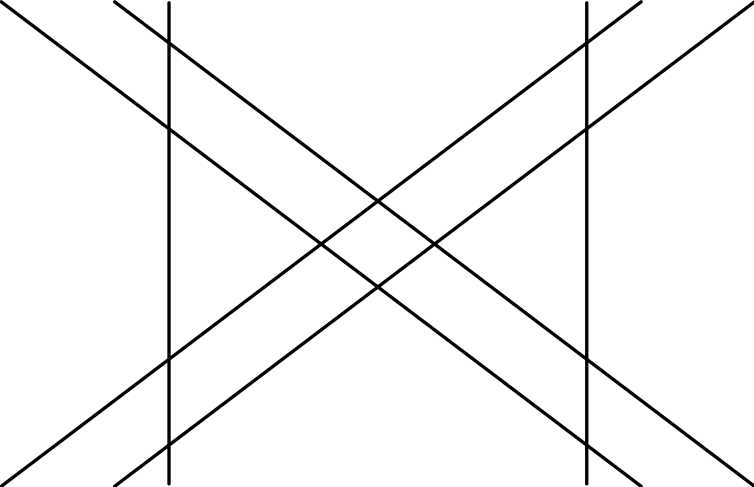
\includegraphics[width=\textwidth]{figures/intro_curves1.png}
    \caption{curves} \label{subfig:intro_unboundedFaces_a}
  \end{subfigure}%
  ~%
  \begin{subfigure}{.32\textwidth}
    
\includegraphics[width=\textwidth]{figures/intro_unboundedFaces_b.png}
    \caption{separate faces} \label{subfig:intro_unboundedFaces_b}
  \end{subfigure}%
  ~%
  \begin{subfigure}{.32\textwidth}
    
\includegraphics[width=\textwidth]{figures/intro_unboundedFaces_c.png}
    \caption{unified face} \label{subfig:intro_unboundedFaces_c}
  \end{subfigure}%
  \caption[xxx]
          {Two approaches for dealing with the unbounded exterior region.
          In this work we take the approach in Figure~\ref{subfig:intro_unboundedFaces_c}, that is to say, treating the whole exterior region as one unbounded face.}
  \label{fig:intro_unboundedFaces}
\end{figure}

\paragraph{Node}
\td{}
\paragraph{Half-edge}
\td{}

%%%%%%%%%%%%%%%%%%%%%%%%%%%%%%%%%%%%%%%%%%%%%%%%%%%%%%%%%%%%%%%%%%%%%%%%%%%%%%%%
\subsection{Background}
\td{I still can't believe this problem has not been solved! :(}
%% Where the space $\mathcal{S}$ is two dimensional and the curve set $\mathcal{C}$ contains the level curves of only linear functions ($f(X)$).
%% \[ \mathcal{C} = \lbrace c_i \mid c_i: ax_1+bx_2+c=0, i \in I, \text{$I$: index set of $\mathcal{C}$} \rbrace \]
%% Consequently every face is a polygon bounded to line segments.


%%%%%%%%%%%%%%%%%%%%%%%%%%%%%%%%%%%%%%%%%%%%%%%%%%%%%%%%%%%%%%%%%%%%%%%%%%%%%%%%
\subsection{This work}

This work aims at studying the subdivision problem in the presence of circles.
After identifying the limitation of the existing solutions in handling the more generic cases, challenges are identified and addressed.
Figure~\ref{fig:intro_curvesPartitioning2} illustrates an example of a planar subdivision in the presence of circles.
This work relies on the following assumptions:
\begin{description}
\item [Dimension] the space is a two dimensional plane.
\item [Curves] the set $\mathcal{C}$ contains levels curves resulted from either linear functions (straight lines as an example of an unbounded class) or conic sections (circles as an example of a bounded class).
\item [Redundancy] if two curves were identical, their intersection would be the same curve which is beyond a finite set of points.
  In order to prevents the intersection procedure yielding a result other than a finite set of points, redundant curves are rejected so that;
  \[ \nexists c_i , c_j \in \mathcal{C}, \quad c_i = c_j \]
\end{description}

\begin{figure}%[!ht]
  \centering
  \begin{subfigure}{.4\textwidth}
    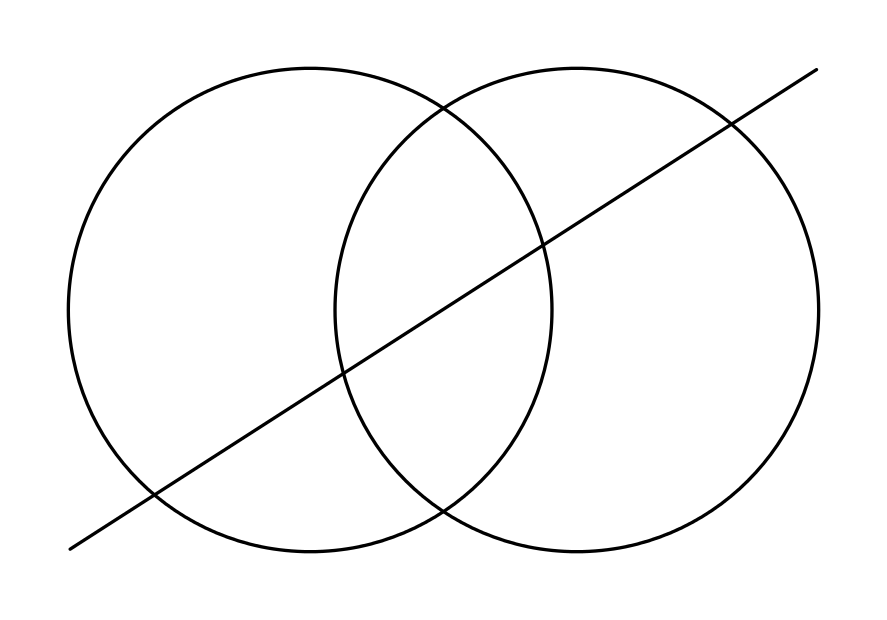
\includegraphics[width=\textwidth]{figures/intro_curves2.png}
    \caption{curves} \label{subfig:intro_curves2}
  \end{subfigure}%
  \quad \quad \quad%
  \begin{subfigure}{.4\textwidth}
    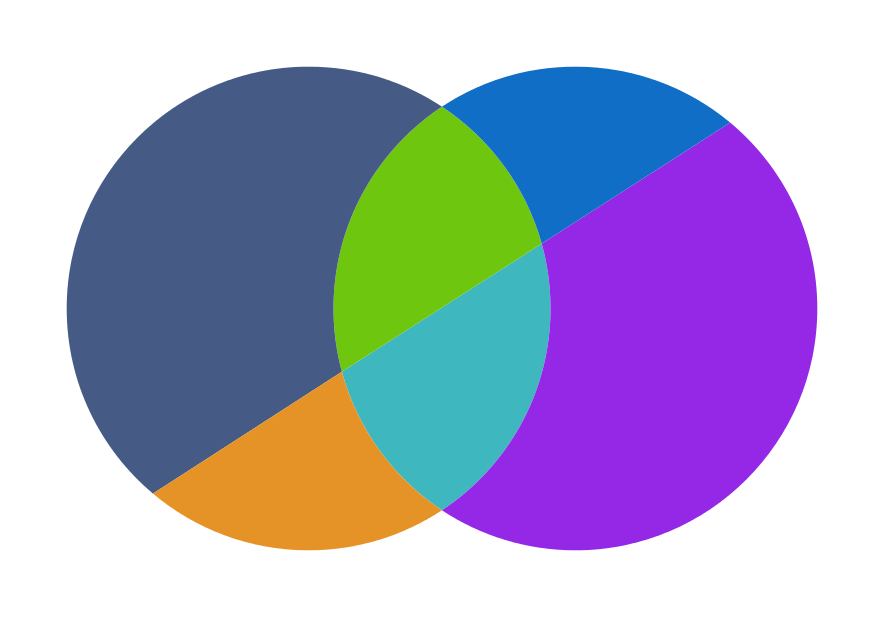
\includegraphics[width=\textwidth]{figures/intro_partitioning2.png}
    \caption{partitioning} \label{subfig:intro_partitioning2}
  \end{subfigure}%
  \caption[xxx]
          {A planar subdivision, over a set of curves containing a straight line and two circles.
          Figure~\ref{subfig:intro_curves2} shows the set of curves, and the ``faces'' resulting from partitioning are color coded in Figure~\ref{subfig:intro_partitioning2}.}
  \label{fig:intro_curvesPartitioning2}
\end{figure}

%%%%%%%%%%%%%%%%%%%%%%%%%%%%%%%%%%%%%%%%
\subsubsection{Challenges}

Introducing circles raises challenges from the meta-algorithm of subdivision, all the way to sub-procedures within.
Most of these challenges, as we'll see, are based on three essential differences between lines and circles;
\begin{inparaenum}[\itshape i\upshape)]
  \item \emph{boundness}: a circle could be enclosed within a closed curve (i.e. a Jordan Curve), while a line stretches to infinity;
  \item \emph{closed curve}: unlike a line, a circle itself is a closed curve and alone could result in bounded faces; and 
  \item \emph{segment representation}: while a segment of a line could be represented by a vector, a segment of a circle is represented by an arc.
\end{inparaenum}


\paragraph{None intersecting circles}
If a line does not intersect with any other curves in the curve set $\mathcal{C}$, it could be safely discarded as it would not result in any bounded region.
On the other hand, a circle which does not have any intersection point with other curves would result in a bounded region that should be counted and identified as a face.
That is to say, in the absence of circles it is safely assumed that the intersection points are well representing all the edges, and consequently all the faces.
We tackle this problem by introducing dummy intersection points over non-intersecting circles.

\paragraph{Sorting nodes over curves}
In order to identify the edges resulting from a curve, it is essential to be able to geometrically sort the intersection points over the curve.
For lines it suffices to sort the points according to their $x$ (or $y$) values.
This does not hold for circles.
To this end, we employ a uni-variate representation for curves (presented in Appendix~\ref{app:alternativeRep}).

\paragraph{Edges are no longer vectors}
A key information in face identification is the ability to follow a geometric path of edges that bound a face.
This is an iterative process of finding the correct successor to an edge, until the sequence of edges form a closed curve, which represents the face.
The correct successor is identified by its departing angle with respect to the arriving angle of the last edge.
In the case of only lines, the arriving and departing angles of edges are equivalent to the slope of the line.
But in the case of arc shaped edges, we have to employ the derivatives of the curve and the intersection point to find the correct successor.

\paragraph{Holes}
A new feature that appears in the presence of circles is the holes.
That is to say, a face could have a non-continuous sequence of edges that define its boundary.
This is due to the face that a circle could be enclosed in the closed curve of a face, and creating a ``hole'' in it.
On the subdivision level, it causes the subdivision to become topologically disconnect (i.e. have separate connected components).
We approach this problem by partitioning the space according to each connected components of the subdivision separately, and merging their results at the end.

\paragraph{Membership function}
Membership function for the subdivision of lines could be implemented through a set of tests relying on cross products, as described in \cite{de2000computational}.
The tests are to check whether if a point is located on the same side of all the bounding edges of a face.
This would only work if the edges could be represented by vectors, and if the face is convex.
As can be seen in Figure~\ref{fig:intro_crossProdFail}, edges turn to arcs in the presence of circles, and potentially a face could be concave.
As an alternative we suggest the use of ``point-in-polygon'' method, which is based upon the Jordan Curve theorem.

\begin{figure} %[!ht]
    \centering
    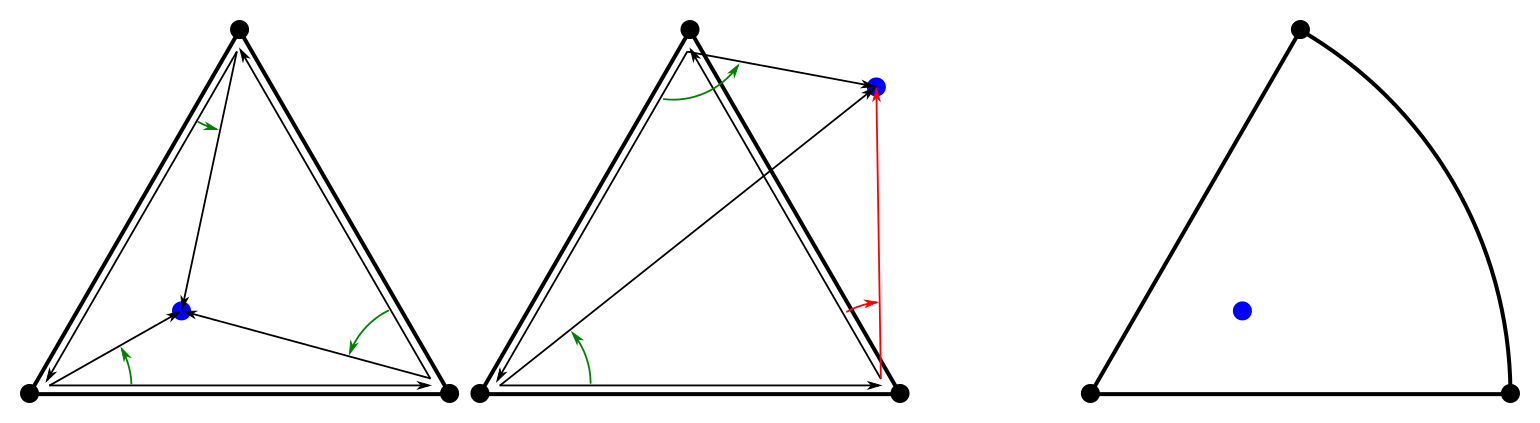
\includegraphics[width=1.\textwidth]{figures/intro_crossProdFail.png}
    \caption{Membership function for the case of only straight lines could be based on tests relying on a cross product.
    However, as the edges are no longer vectors in the presence of circles, the conventional membership procedure requires revision.}
    \label{fig:intro_crossProdFail}
\end{figure}

\section{Subdivision}
The process of our method for constructing the subdivion is explained in this section.
The core process of subdivion is the decomposition of the space into faces, according to a provided set of curves.
That is to say, identifying every individual face.
On the other hand, in order to satisfy the required functionality of the resulting subdivion (such as membership function and neighbourhood function), proper descriptions of intermediate and underlying data structures are essential.
Such descriptions will be provided in the appendix~\ref{app:datastructure}.\bigskip

Algorithm~\ref{alg:subdivisionRestricted} presents a restricted version of the subdivision construction algorithm.
While explaining the sub-procedures mentioned in algorithm~\ref{alg:subdivisionRestricted}, the restrictions and their remedy would be described.
A more comprehensive version of algorithm~\ref{alg:subdivisionRestricted} will be presented afterward.

\begin{algorithm}
  \caption {Subdivision (restricted version)}
  \label{alg:subdivisionRestricted}
  \begin{algorithmic}    
    \STATE INPUT  $\mathcal{C}:\{curves\}$
    \STATE OUTPUT  $\mathcal{F}:\{faces\}$
    \STATE \quad
    \STATE $\mathcal{N}:\{nodes\} = \mathit{intersect} \left( \mathcal{C} \right)$
    \STATE $\mathcal{E}:\{half\text{-}edges\} = \mathit{segment} \left( \mathcal{C}, \mathcal{N} \right)$
    %% \STATE Construct a Multi Directional Graph ($\mathit{MDG}$) from $\left( \mathcal{E}, \mathcal{N} \right)$
    %% \STATE $ \mathcal{F}=\{faces\} = \mathit{partition} \left( \mathit{MDG} , \mathcal{C} \right)$
    %% \STATE return $\mathit{Subdivision}\left( \mathcal{C},\mathcal{F}, \mathit{MDG} \right)$
    \STATE $ \mathcal{F}:\{faces\} = \mathit{partition} \left(\mathcal{C},\mathcal{E} \right)$
  \end{algorithmic}
\end{algorithm}

Algorithm~\ref{alg:subdivisionRestricted}, which is quite identical to the subdivision algorithm presented in \cite{de2000computational}, is demonstrated in figure~\ref{fig:subd_simpleExample}.
It should be reiterate that the focus of this work is to revise the meta-algorithm and its sub-procedures, so that it can handle the more general cases including curves of circle class.
Regardless, we first try to provide an intuitive and basic understanding of the restricted version, and in the following sections we'll provides details on the computation and required extensions to each procedure.
The objective of the restricted version of the subdivision algorithm (presented in algorithm~\ref{alg:subdivisionRestricted} and demonstrated in figure~\ref{fig:subd_simpleExample}) is to identify those partitioned areas of the space (denoted by $\mathcal{S}$) into a set of faces (denoted by $\mathcal{F}$.)
The first step is to find the set all the intersection points bewteen all the curves (figure~\ref{subfig:subd_simpleExample_b}).
This set is denoted by $\mathcal{N}$, standing for \emph{nodes} \footnote{The reason for the name is the important role that they play in constructing a graph in the extended version of the algorithm. Eventhough we'll come to this aspect later, we use the same term for consistency.}.
Every node resulting from this process is also assigned to the curves that yielded it.
For the next step, that is segmenting curves into half-edge based on their nodes, it is important that the nodes' assigments to the curves should be geometrically sorted over curves.
In the case of only straight line, the sorting process is performed by looking at the $x$ (or $y$) values of the nodes.
A more comprehensive approach for sorting will be presented later in section~\ref{subsec:halfEdgeConstruction}.
After sorting the nodes over each curve, the curves are segmented to edges as illustrated in figure~\ref{subfig:subd_simpleExample_c}.
Note that each simple edge is composed of two ``twin'' directed half-edges, represented by blue vectors in figure~\ref{subfig:subd_simpleExample_c}.
For more detail on half-edge data structure please see \cite{de2000computational}, or the appendix~\ref{app:datastructure}.
In the final stage, we attend to construct the set of faces $\mathcal{F}$, through a process of path following.
The process starts by fetching (and removing) a half-edge from an open list, moving it to the list
of a face's boundary.
The next member of the face's boundary list is the half-edge that follows the last last in the list.
The potential candidates for the next member are those half-edge who start from the node which the last half-edge of the list is arriving at.
The next element is identified among the candidates by measuring their angles to the last half-edge.
The one with widest Counter Clock-Wise (CCW) angle with respect to the last half-edge is identified as the new member of the face's boundary list.
As we will see later, this conventional method for following the boundary of a face would fail in the presence of curves from circle classes, for which we provide other measures from first and second derivatives of the curves.

\begin{figure}%[!ht]
  \centering
  \begin{subfigure}{.4\textwidth}
    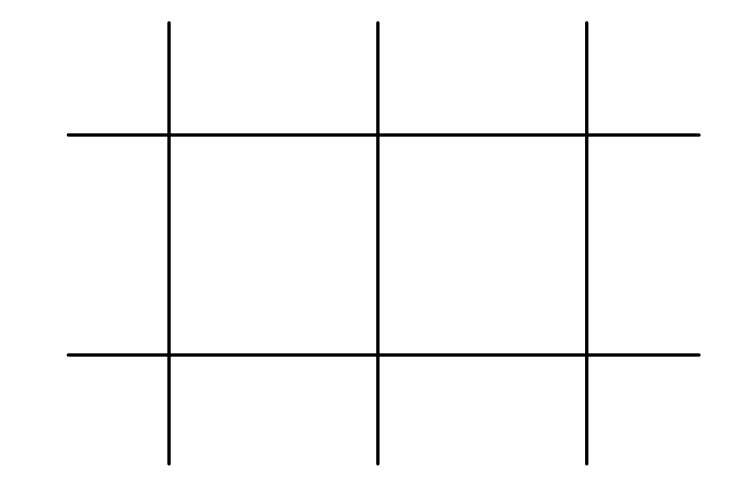
\includegraphics[width=\textwidth]{figures/subd_simpleExample_a.png}
    \caption{$\mathcal{C}$: curves} \label{subfig:subd_simpleExample_a}
  \end{subfigure}%
  \quad \quad%
  \begin{subfigure}{.4\textwidth}
    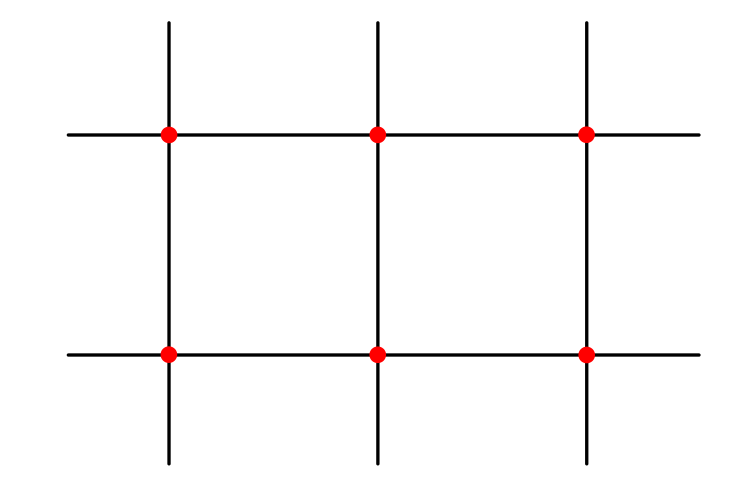
\includegraphics[width=\textwidth]{figures/subd_simpleExample_b.png}
    \caption{$\mathcal{N}$: nodes} \label{subfig:subd_simpleExample_b}
  \end{subfigure}

  \begin{subfigure}{.4\textwidth}
    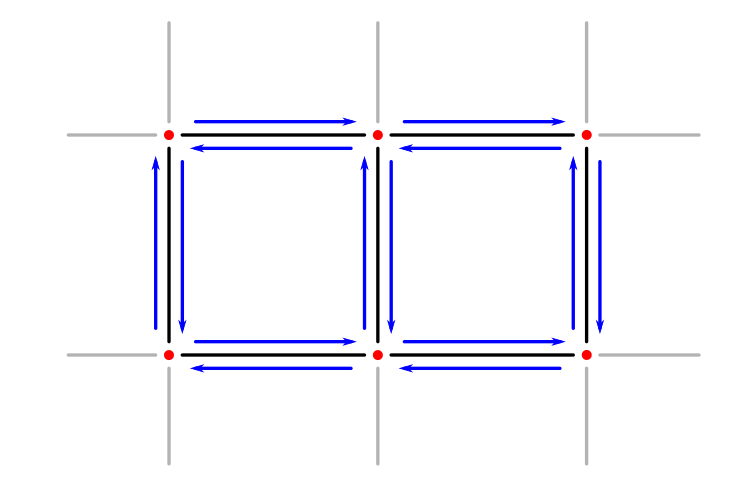
\includegraphics[width=\textwidth]{figures/subd_simpleExample_c.png}
    \caption{$\mathcal{E}$: half-edges} \label{subfig:subd_simpleExample_c}
  \end{subfigure}%
  \quad \quad%
  \begin{subfigure}{.4\textwidth}
    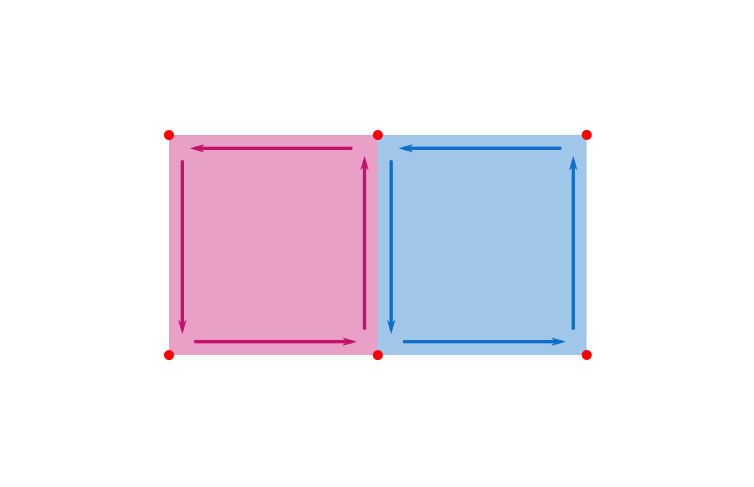
\includegraphics[width=\textwidth]{figures/subd_simpleExample_d.png}
    \caption{$\mathcal{F}$: faces} \label{subfig:subd_simpleExample_d}
  \end{subfigure}%
  \caption[xxx]
          {A simplified demonstration of the subdivision algorithm.}
  \label{fig:subd_simpleExample}
\end{figure}


%%%%%%%%%%%%%%%%%%%%%%%%%%%%%%%%%%%%%%%%%%%%%%%%%%%%%%%%%%%%%%%%%%%%%%%%%%%%%%%%
\subsection{Intersection procedure}
This procedure, as presented in algorithm~\ref{alg:intersectionProcedure}, intersects all curves with each other.
Each intersection point (node as we call them) will be assigned to curves which it is yielded from.
Furthermore, different curves might intersect at the same location, resulting in duplication of the points.
The procedure overcomes this problem by removing redundant points while updating the assignment of points to curves.

\begin{algorithm}
  \caption {Intersect: curve intersection procedure}
  \label{alg:intersectionProcedure}
  \begin{algorithmic}    
    \STATE INPUT  $\mathcal{C}:\{curves\}$
    \STATE OUTPUT  $\mathcal{N}:\mathit{nodes}$
    \STATE \quad
    %% \STATE [step2] find all intersections
    \STATE $\mathcal{N} = \emptyset$
    \FORALL {$curve_i, curve_j \in \mathcal{C} \mid i>j$}
    \STATE $\{nodes\}=intersect\left( curve_i, curve_j \right) $
    \FORALL {$node_k \in \{nodes\}$}
    \STATE append $node_k$ to $\mathcal{N}$
    \STATE assign $node_k$ to $curve_i$ and $curve_j$
    \ENDFOR
    \ENDFOR
    \STATE \quad
    %% \STATE [step3] remove redundancy
    \FORALL {$node_i, node_j \in \mathcal{N} \mid i \neq j, distance(node_i,node_j)=0$}
    \STATE assign $node_i$ to all curves that $node_j$ is assigned to
    \STATE dump $node_j$ from $\mathcal{N}$
    \ENDFOR
  \end{algorithmic}
\end{algorithm}

%%%%%%%%%%%%%%%%%%%%%%%%%%%%%%%%%%%%%%%%
\paragraph{Non-intersecting Circles}
The result of intersection procedure is the ground for identifying half-edges (as detailed in the next section).
Each curve is segmented into half-edges, according to those nodes that are placed on them.
In the presence of circles, there is a chance that a circle might not be intersecting with any other curve.
Consequently no half-edges would be identified on that circle.
We tackle this problem by placing a \emph{pseudo} intersection point on the circle's curve at an arbitrary location, resulting in a node that is only assigned to one curve (i.e. the non-intersecting circle.)

%%%%%%%%%%%%%%%%%%%%%%%%%%%%%%%%%%%%%%%%%%%%%%%%%%%%%%%%%%%%%%%%%%%%%%%%%%%%%%%%
\subsection{Half-Edge identification} \label{subsec:halfEdgeConstruction}

Following the algorithm~\ref{alg:intersectionProcedure}, every intersection point (node) lying on every curve is provided.
Algorithm~\ref{alg:halfedgeConstruction} describes the process of segmenting each curve into half-edges that connect nodes to each other.
Such information are essential for the next step of the algorithm~\ref{alg:subdivisionRestricted}, i.e. face identification (and graph construction in the complete version of the algorithm.)\bigskip

This step of the algorithm requires the ability to sort nodes over each curve.
As mentioned earlier, in the case of only straight line, the sorting process is performed by looking at the $x$ (or $y$) values of the nodes.
This would clearly fail in the presence of circles.
To this end, we employ an alternative representation of the level-curves (denoted by $\dot{f}$), as a function of a single variable $\theta$, that traverses over the level-curve of the multivariable function\footnote{The equations are presented in appendix~\ref{app:alternativeRep}.}.
Given the ``alternative'' representation of a level-curve as a function of a single variable $\theta$, we use the inverse function of it (denoted by $\dot{f}^{-1}$), to sort nodes over the curve ($\theta = \dot{f}^{-1}(x,y)$).
Provided that it's possible to sort nodes over the curves, we can proceed with the algorithm~\ref{alg:halfedgeConstruction} which describes the construction of half-edges.
Figure~\ref{fig:subd_heConstruct} demonstrates two examples of half-edge construction over a line and a circle.
The algorithm~\ref{alg:halfedgeConstruction} takes segments of the curve under process and turns each segment into two twin half-edges.
The segments are identified by the consecutive nodes over the curve.

\begin{figure}
    \centering
    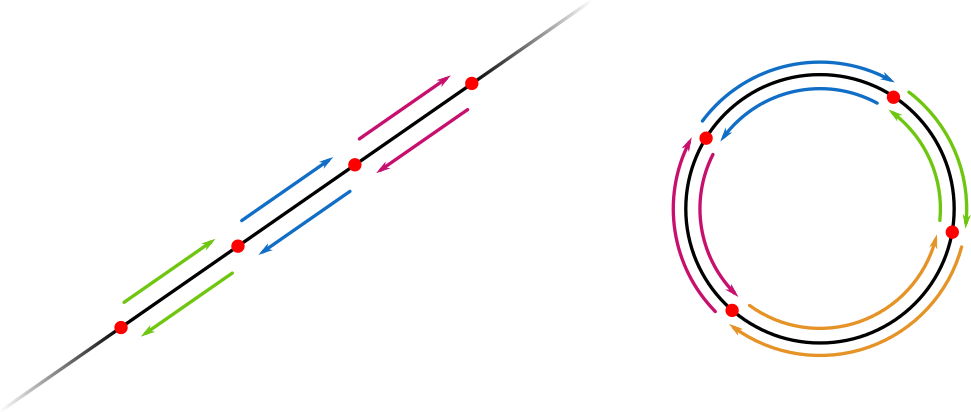
\includegraphics[width=.8\textwidth]{figures/subd_heConstruct.png}
    \caption{Examples of half-edge construction over a line and a circle.
      In each case, half-edges with the same color are twins.}
    \label{fig:subd_heConstruct}
\end{figure}

\begin{algorithm}
  \caption {Segment: half-edge construction}
  \label{alg:halfedgeConstruction}
  \begin{algorithmic}
    \STATE INPUT  $\mathcal{C}:\{curves\}, \quad \mathcal{N}:\{nodes\}$
    \STATE OUTPUT  $\mathcal{E}:\{half\text{-}edges\}$
    \STATE \quad
    \STATE $\mathcal{E} = \emptyset$
    \FORALL {$curve_i \in \mathcal{C}$}
    \STATE $list\_n = \{node_j \mid node_j \in \mathcal{N}, node_j \text{ is assigned to } curve_i \}$
    \STATE sort the $list\_n$ according to $\theta_j=\dot{f}_{i}^{-1}(node_j)$
    \STATE $I= \text{index set of the } list\_n$
    \STATE $list\_he=\left\{(curve_i,node_j,node_{j+1}),(curve_i,node_{j+1},node_j) \mid \forall j \in I \right\}$
    \IF {$curve_i$ is a circle}
    \STATE $j=max(I)$
    \STATE append $\{(curve_i,node_j,node_{0}),(curve_i,node_0,node_{j})\}$ to $list\_he$
    \ENDIF
    \STATE append $list\_he$ to $\mathcal{E}$
    \ENDFOR    
  \end{algorithmic}
\end{algorithm}


%%%%%%%%%%%%%%%%%%%%%%%%%%%%%%%%%%%%%%%%%%%%%%%%%%%%%%%%%%%%%%%%%%%%%%%%%%%%%%%%
\subsection{Partitioning procedure: face identification}
%% When t is increasing, the half-edge is positive, for any curve. Very important to understand the code.
Identification of faces is performed by a procedure of path following.
Given that each half-edge belongs to only one face, the process start by picking an arbitrary half-edge and detecting the boundary of the face it belongs to, by picking the correct successor to the last half-edge.
This is an iterative process that terminats when the last half-edge arrives at the node which the first half-edge started from.
This procedure is represented by algorithm~\ref{alg:partitioning} and demonstrated in figure~\ref{fig:subd_pathFollower}.

\begin{algorithm}
  \caption {Partition: face identification}
  \label{alg:partitioning}
  \begin{algorithmic}
    \STATE INPUT  $\mathcal{C}:\{curves\}, \quad \mathcal{N}:\{nodes\}, \quad \mathcal{E}:\{half\text{-}edges\}$
    \STATE OUTPUT  $\mathcal{F}:\{faces\}$
    \STATE \quad
    \STATE $\mathcal{F} = \emptyset$
    \STATE $open\_list = \mathcal{E}$
    \WHILE{$open\_list \neq \emptyset$}
    \STATE fetch a random $half\_edge_i$ and remove it from $open\_list$
    \STATE $face\_list = \{ half\_edge_i\}$
    \STATE $start\_node = node_s$, where $half\_edge_i$ departs from $node_s$
    \STATE $end\_node = node_e$, where $half\_edge_i$ arrives at $node_e$
    \WHILE{$start\_node \neq end\_node$}
    \STATE $half\_edge_j= \mathit{find\_successor} \left( \text{last } half\_edge \text{ in } face\_list \right)$
    \STATE remove $half\_edge_j$ from $open\_list$ and add it to $face\_list$
    \STATE update $end\_node$ according to $half\_edge_j$
    \ENDWHILE
    \STATE construct a face instance from $face\_list$ and append it to $\mathcal{F}$
    \ENDWHILE
  \end{algorithmic}
\end{algorithm}

\begin{figure} %[!ht]
    \centering
    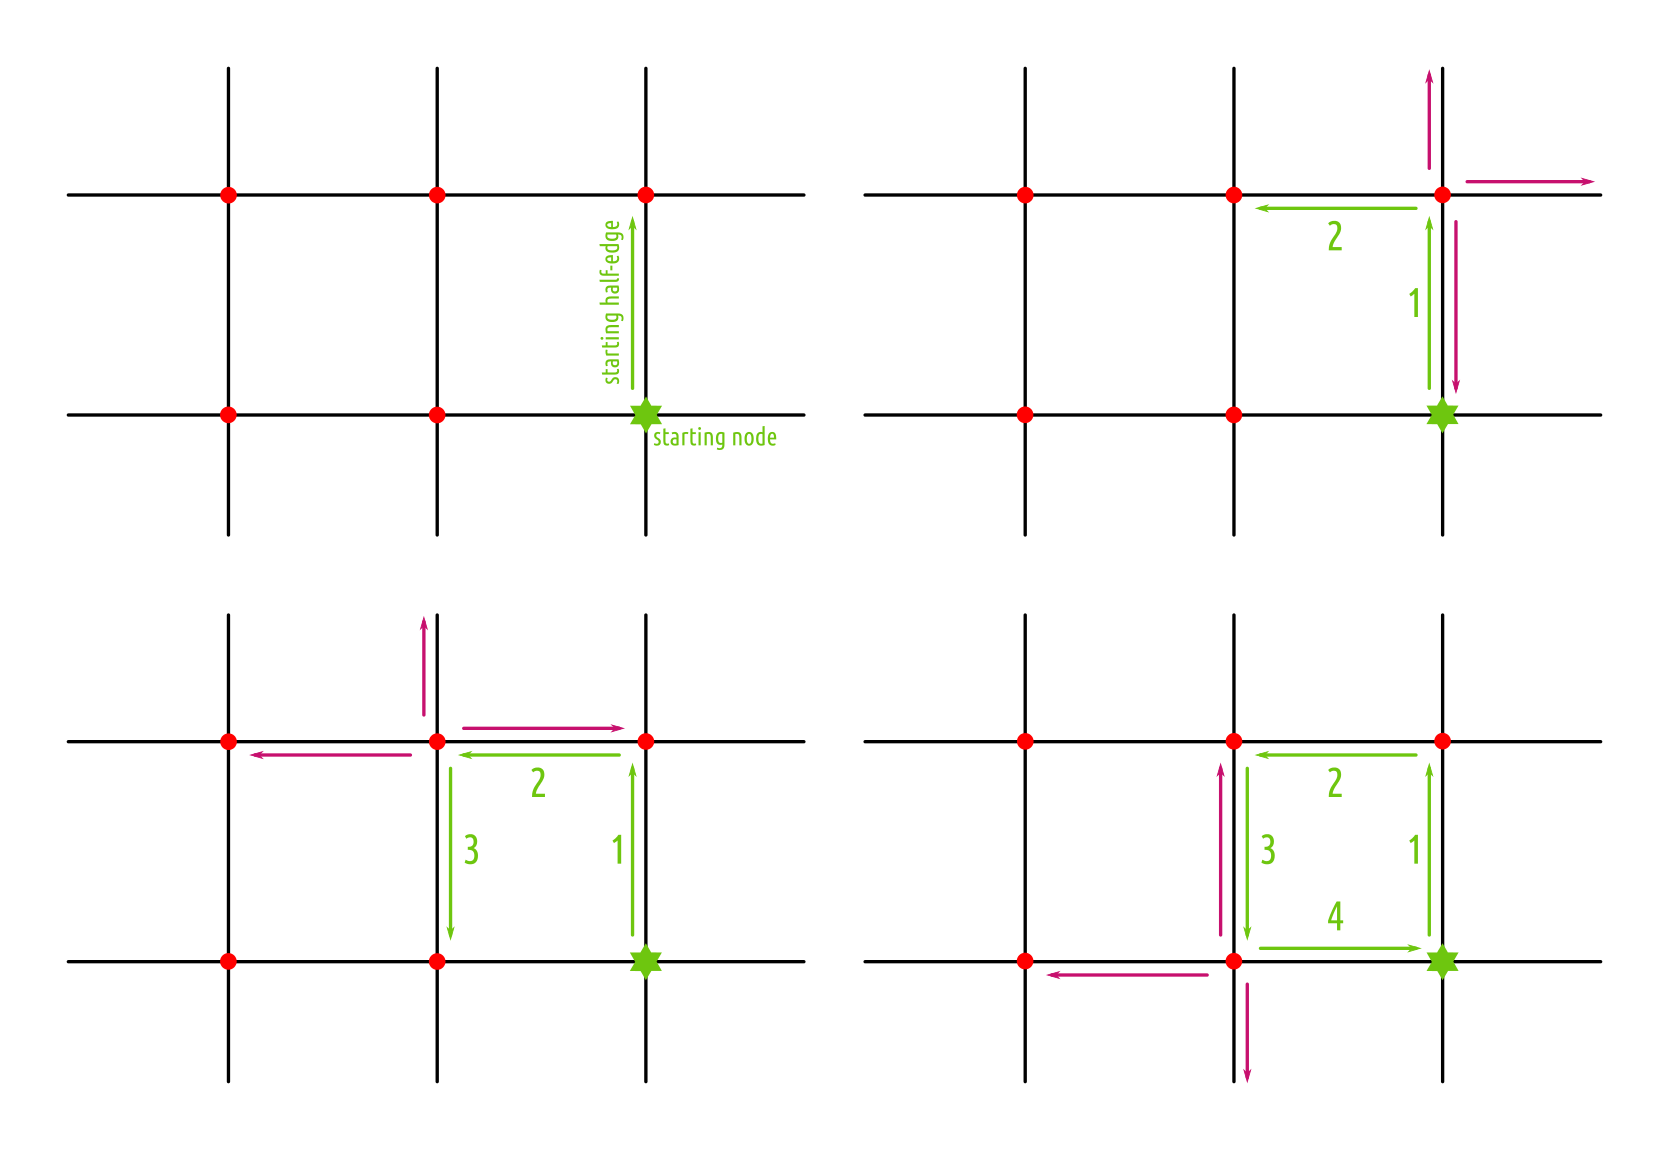
\includegraphics[width=1.\textwidth]{figures/subd_pathFollower.png}
    \caption{The process of face identification towards partitioning.
      First a half-edge is picked, which initiats the identification of a new face.
      Then the correct successor (colored green) is identified among candidates.
      Rejected candidates at each step are colored red.
      The process terminates, and the face is completely identified, when the last half-edge arrives at the starting node of the first half-edge.}
    \label{fig:subd_pathFollower}
\end{figure}

%%%%%%%%%%%%%%%%%%%%%%%%%%%%%%%%%%%%%%%%
\subsubsection{Finding the correct successor half-edge}

Half-edges departing from the node, which last half-edge of the face arrived at, are flagged as candidates.
Among the candidates, the twin of the last half-edge is rejected.
The winning candidate is the one with widest departing angle (CCW) with respect to the departing angle of the last half-edge's twin.
That is to say, the half-edge that is closest to the twin's departure.
Few examples of correct successor selections are demonstrated in figure~\ref{fig:subd_findNextHalfEdge}, where the arriving half-edges and the correct successors are colored green, and all the rejected candidates are colored red.

\begin{figure}%[!ht]
  \centering
  \begin{subfigure}{.32\textwidth}
    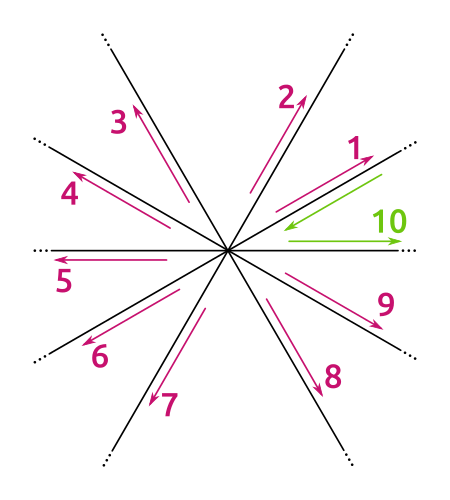
\includegraphics[width=\textwidth]{figures/subd_findNextHalfEdge_a.png}
    \caption{only straight lines} \label{subfig:subd_findNextHalfEdge_a}
  \end{subfigure}%
  ~%
  \begin{subfigure}{.32\textwidth}
    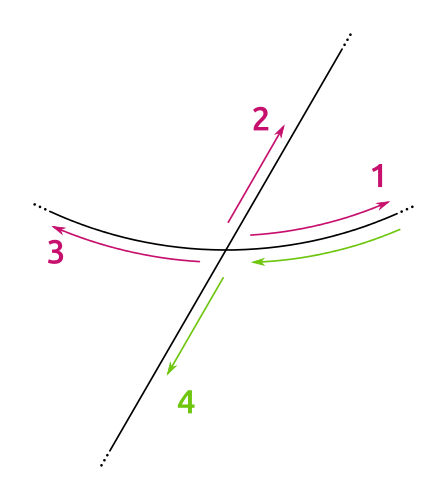
\includegraphics[width=\textwidth]{figures/subd_findNextHalfEdge_b.png}
    \caption{a line and circles} \label{subfig:subd_findNextHalfEdge_b}
  \end{subfigure}%
  ~%
  \begin{subfigure}{.32\textwidth}
    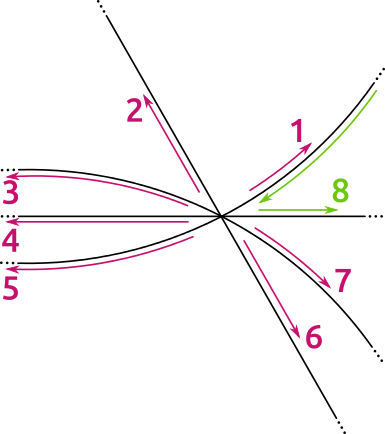
\includegraphics[width=\textwidth]{figures/subd_findNextHalfEdge_c.png}
    \caption{a line and circles} \label{subfig:subd_findNextHalfEdge_c}
  \end{subfigure}%
  \caption[xxx]
          {Few examples of correct successor selections.
            Arriving half-edges and the correct successors are colored green, and all the rejected candidates are colored red.}
  \label{fig:subd_findNextHalfEdge}
\end{figure}

In cases of only straight lines (e.g. figures~\ref{subfig:subd_findNextHalfEdge_a}), finding the next half-edge would be simply to look at candidate half-edges' angles, as half-edges are vectors.
However this does not hold in the presence of circles where half-edges are arcs (see figures~\ref{subfig:subd_findNextHalfEdge_b} and \ref{subfig:subd_findNextHalfEdge_c}.)
To overcome this problem, we rely on the angle of the tangent vector to the level-curves\footnote{The equations for the derivatives are available in appendix~\ref{app:alternativeRep}.}.
These vectors provide the departing and arriving angles of half-edges at the nodes' location.


%% In figure~\ref{fig:subd_derivatives}, the derivatives (red vectors) and their normal (green vectors) are illustrated alongside with the multi-variable functions (gray surfaces) and the level-curves (dashed balck lines.)
%% \begin{figure}%[!ht]
%%   \centering
%%   \begin{subfigure}{.49\textwidth}
%%     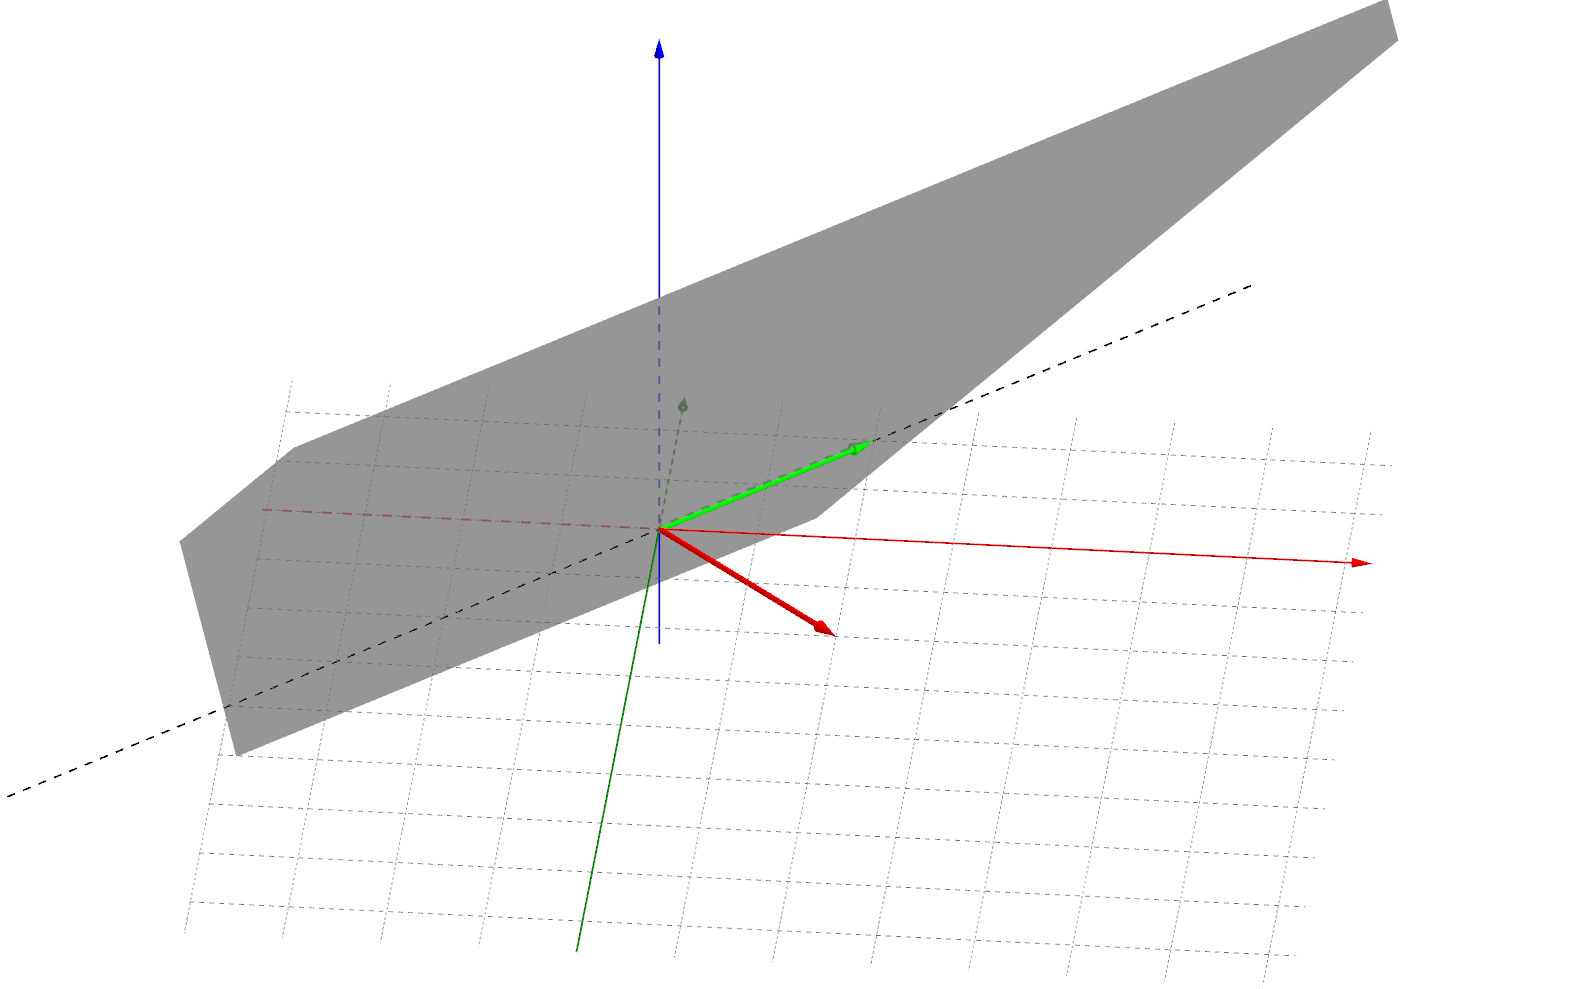
\includegraphics[width=\textwidth]{figures/subd_derivativeLine.png}
%%     \caption{$f\left(x, y\right) = x - y$} \label{subfig:subd_derivativeLine}
%%   \end{subfigure}%
%%   ~%
%%   \begin{subfigure}{.49\textwidth}
%%     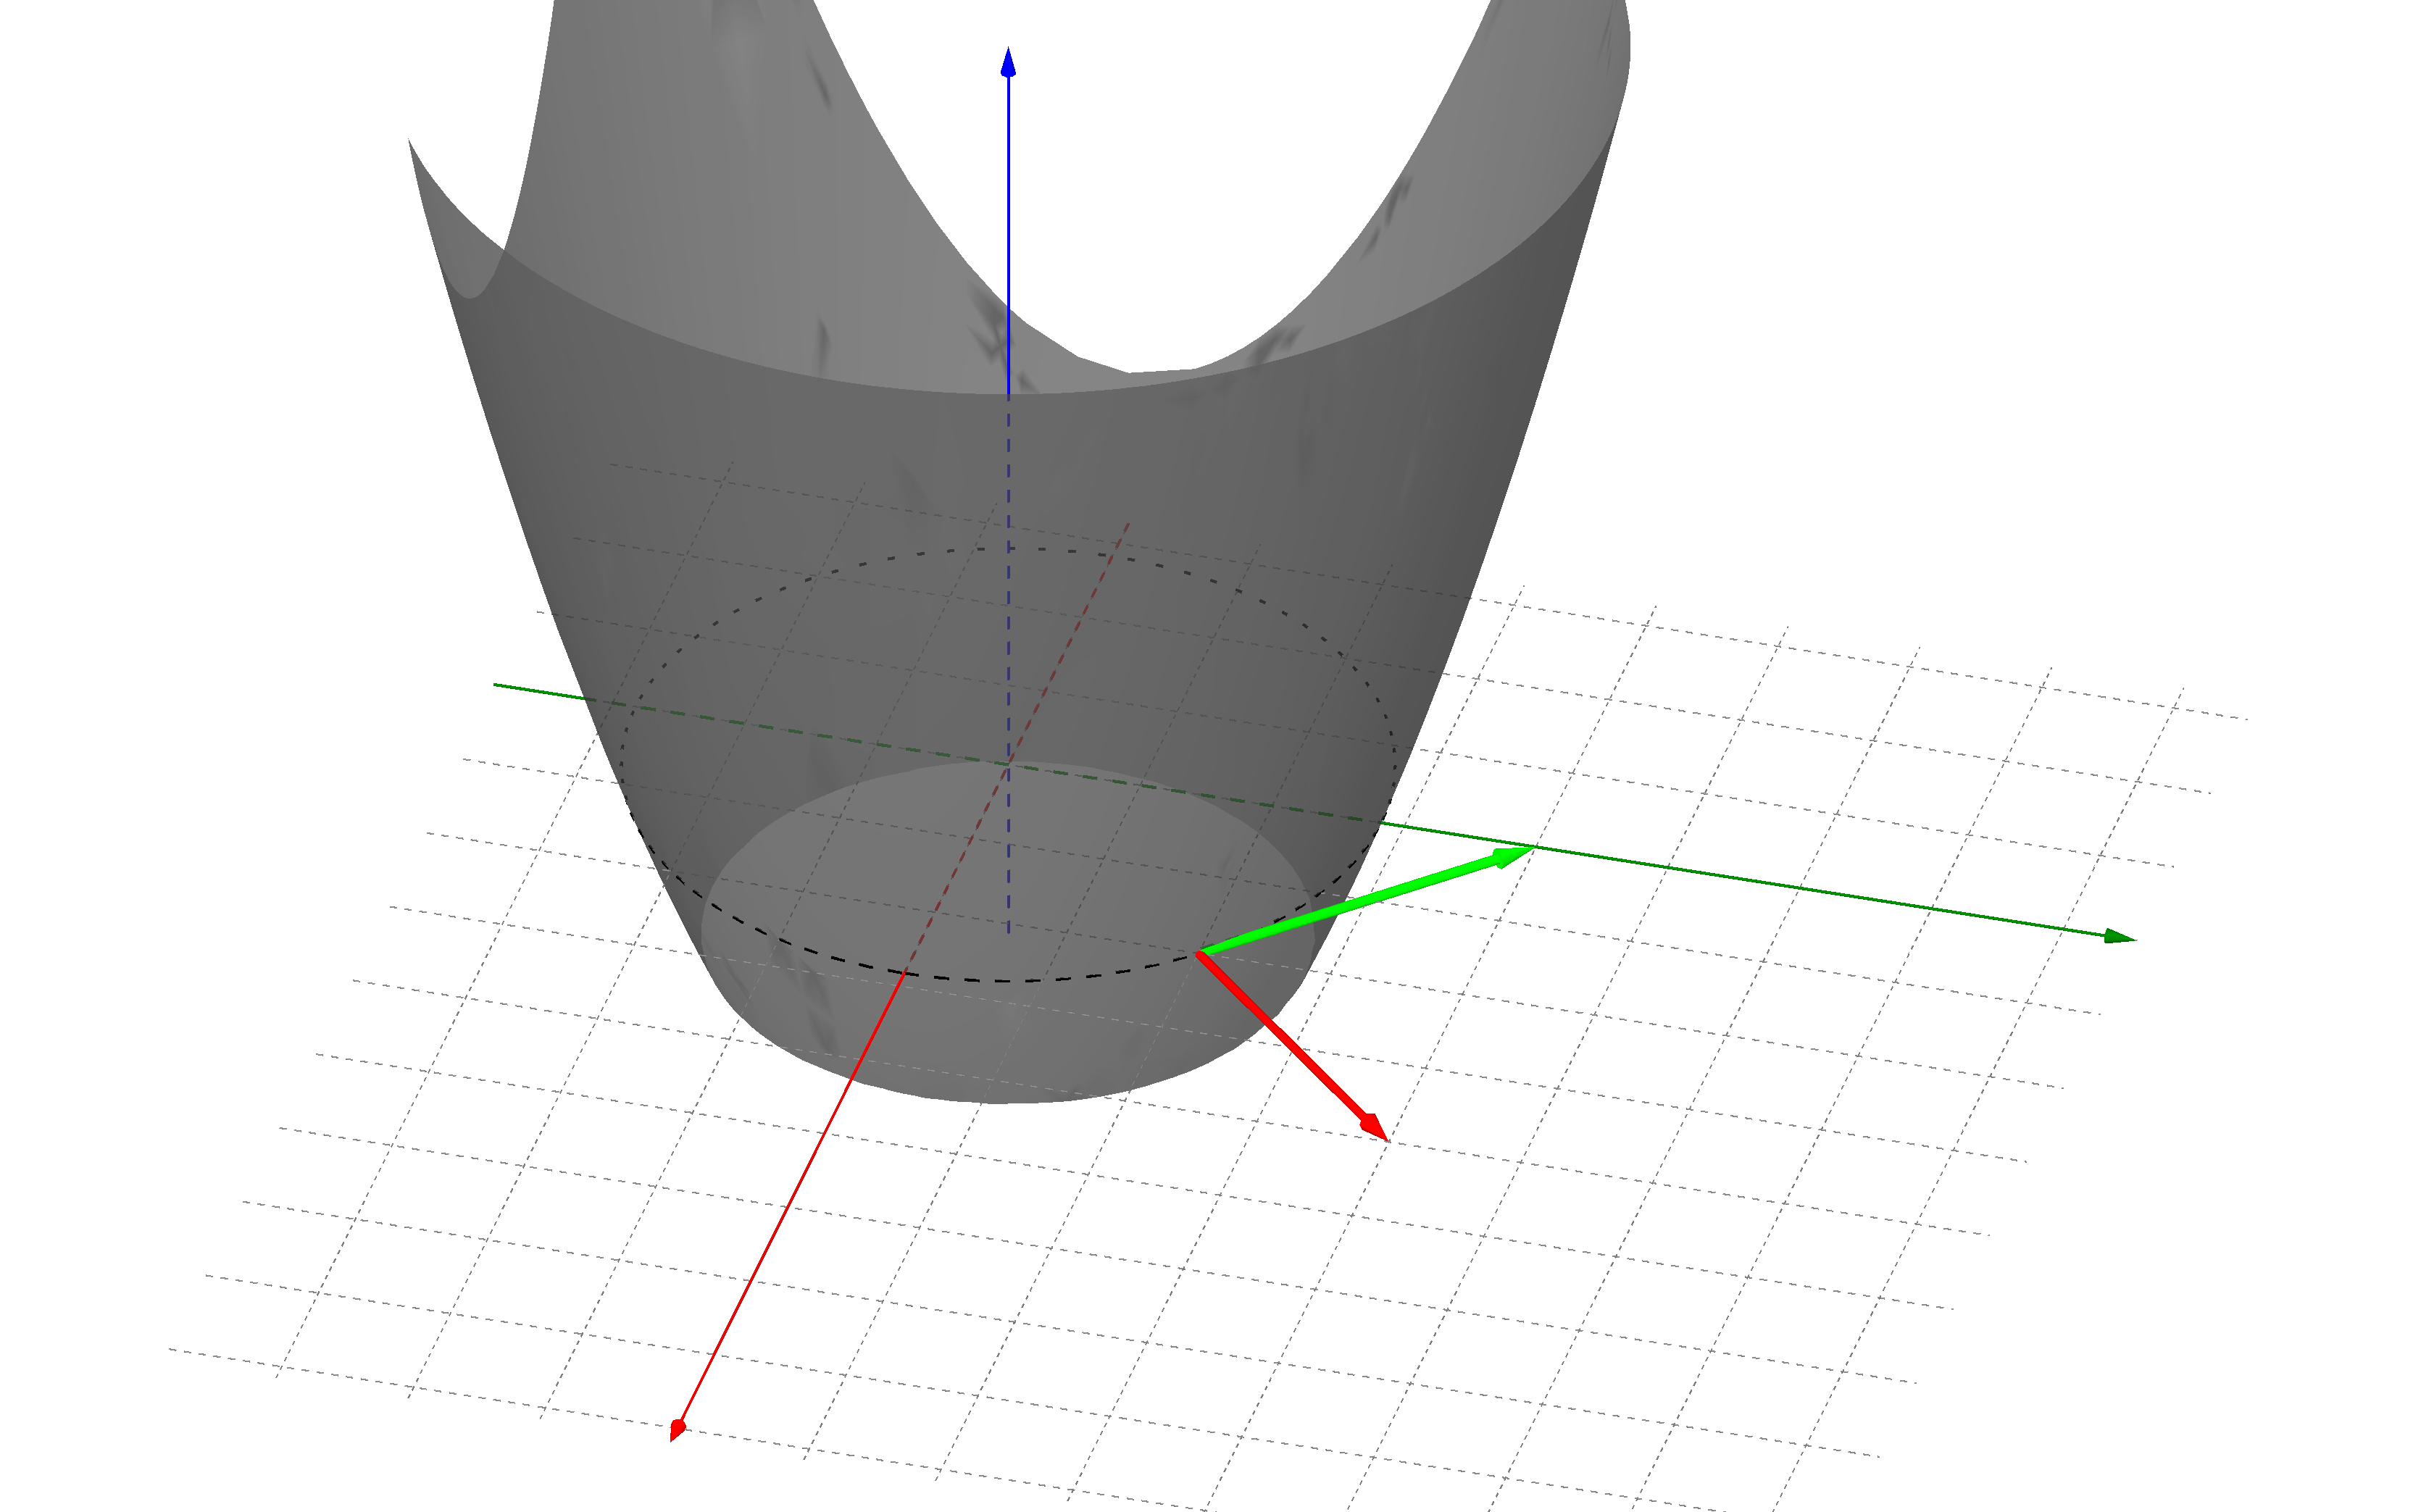
\includegraphics[width=\textwidth]{figures/subd_derivativeCircle.png}
%%     \caption{$f\left(x, y\right) = x^2+y^2-2$} \label{subfig:subd_derivativeCircle}
%%   \end{subfigure}%
%%   \caption[xxx]
%%           {Multi-variable functions as gray surfaces, and their level-curves ($f\left(x, y\right) =0$) in dashed balck lines.
%%             The derivatives are shown as red vectors and their normal vectors are colored green.}
%%   \label{fig:subd_derivatives}
%% \end{figure}

%%%%%%%%%%%%%%%%%%%%%%%%%%%%%%%%%%%%%%%%
\subsubsection{Insufficiency of the first derivative in case of tangency}

When curves intersect while being tangent, the measure of first derivatives' angle at the intersection point is not sufficient to detect the correct successor.
This challenge is demonstrated in figure~\ref{subfig:subd_tangentCase_a} where four circles intersect at a tangent point.
While the correct successor is colored green after the arriving half-edge, one can see that there are two other candidates (neglecting the twin of arriving half-edge) that have the same departing angle at the intersection point as the correct successor.\bigskip

\begin{figure} %[!ht]
    \centering
  \begin{subfigure}{.49\textwidth}
    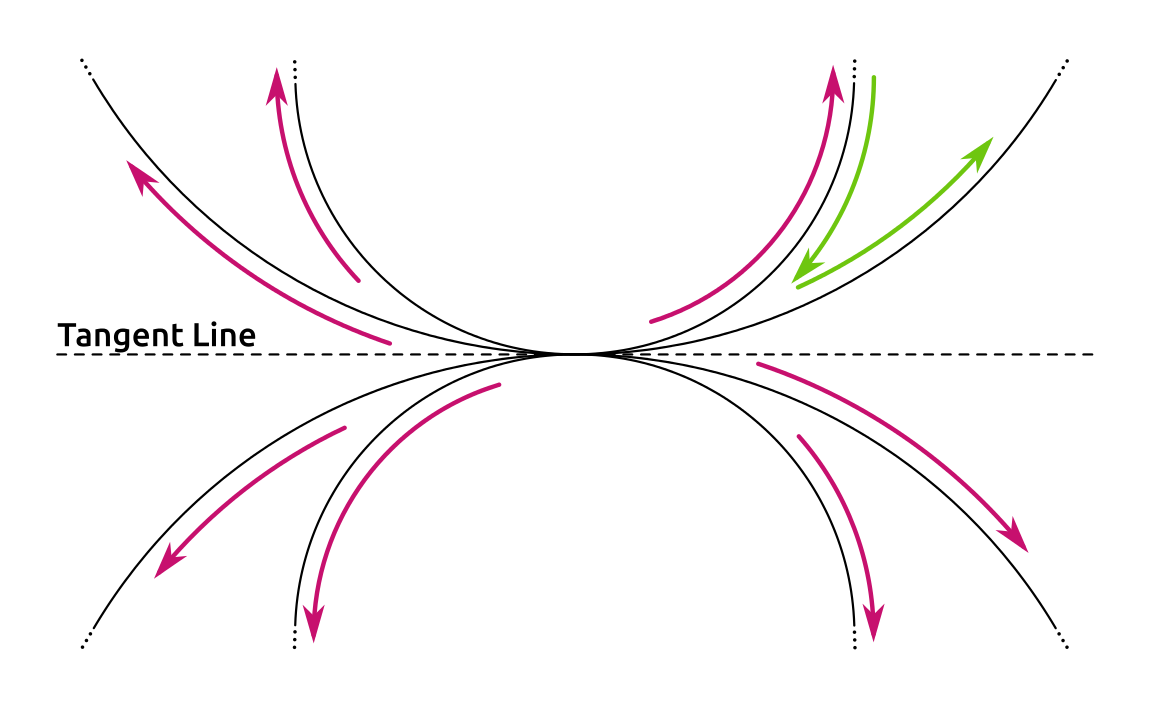
\includegraphics[width=\textwidth]{figures/subd_tangentCase_a.png}
    \caption{a case of tangency} \label{subfig:subd_tangentCase_a}
  \end{subfigure}%
  ~%
  \begin{subfigure}{.49\textwidth}
    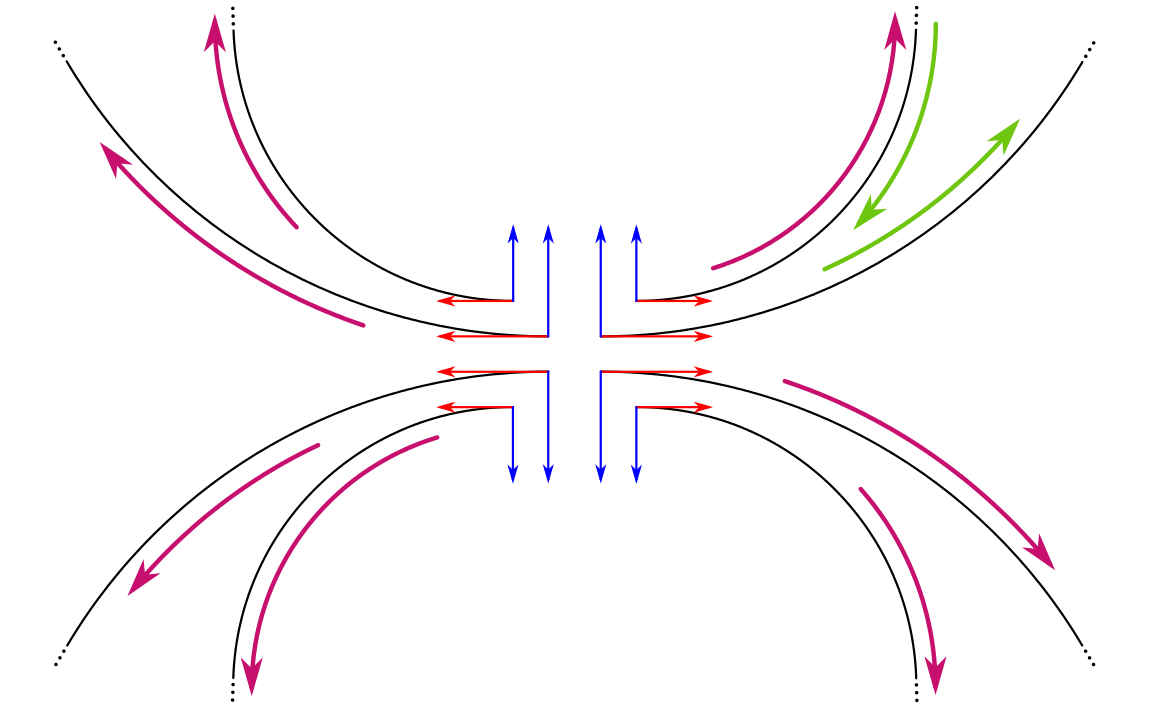
\includegraphics[width=\textwidth]{figures/subd_tangentCase_b.png}
    \caption{derivatives of \emph{half-edges}} \label{subfig:subd_tangentCase_b}
  \end{subfigure}%

    \caption{Curves that intersect, but do not intercept.
      When curves intersect while being tangent, the measure of first derivatives' angle at the intersection point is not sufficient to detect the correct successor.
      A second measure for sorting the cadidates half-edges are provided based on both the first and second derivatives.}
    \label{fig:subd_tangentCase}
\end{figure}

We tackle this problem by adding a secondry sorting measure that relies on both first and second derivatives of the curve at the intersection point\footnote{The equations for the derivatives are available in appendix~\ref{app:alternativeRep}.}.

\[
\begin{array}{l}
  key_1 = \measuredangle \overrightarrow{\frac{d\dot{f}(\theta)}{d\theta}}\\
  \quad\\
  key_2 = \overrightarrow{\frac{d^2\dot{f}(\theta)}{d\theta^2}} \cdot \frac{\overrightarrow{V}}{\|\overrightarrow{V}\|} \quad \text{where: } \overrightarrow{V} = (-y,x) \quad , (x,y) = \overrightarrow{\frac{d\dot{f}(\theta)}{d\theta}}\\
\end{array}
\]

If the $key_1$ is not sufficient to detect the correct successor, that is to say in the tangent case,
the second derivative brings a measure of in which direction, the curve is changing its \emph{course}.
Along with a measure of the first derivative, this change of ``course'' that is delivered by the second derivative makes up the $key_2$.

%%%%%%%%%%%%%%%%%%%%%%%%%%%%%%%%%%%%%%%%%%%%%%%%%%%%%%%%%%%%%%%%%%%%%%%%%%%%%%%%
\subsection{Resolving the restriction} \label{subsec:}

So far we have presented modified versions of the sub-procedures in algorithm~\ref{alg:subdivisionRestricted}, so that they can handle curves beyond straight lines (i.e. circles.)
However this does not suffice, since the algorithm~\ref{alg:subdivisionRestricted} itself would fail in the presence of circles.
Figure~\ref{fig:subd_restrictedFail} show examples of where the ``restricted'' algorithm would fail.
These failures occure when some curves are located inside other faces without intersecting with them.
As a consequence, those insider curves are not accounted for in the entailing faces as there is not connected path between the two.

\begin{figure}%[!ht]
  \centering
  \begin{subfigure}{.32\textwidth}
    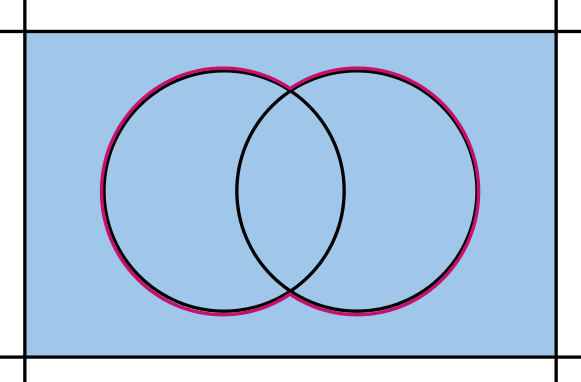
\includegraphics[width=\textwidth]{figures/subd_restrictedFail_a.png}
    %% \caption{xxx} \label{subfig:subd_restrictedFail_a}
  \end{subfigure}%
  ~%
  \begin{subfigure}{.32\textwidth}
    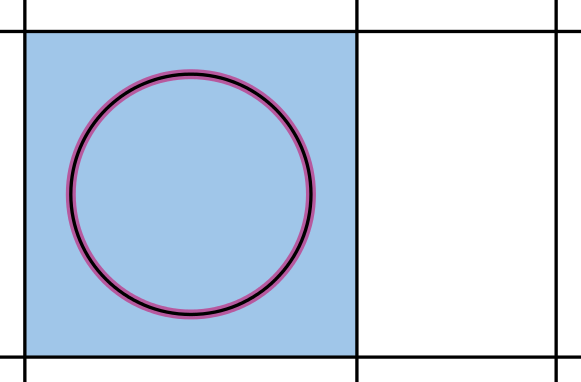
\includegraphics[width=\textwidth]{figures/subd_restrictedFail_b.png}
    %% \caption{xxx} \label{subfig:subd_restrictedFail_b}
  \end{subfigure}%
  ~%
  \begin{subfigure}{.32\textwidth}
    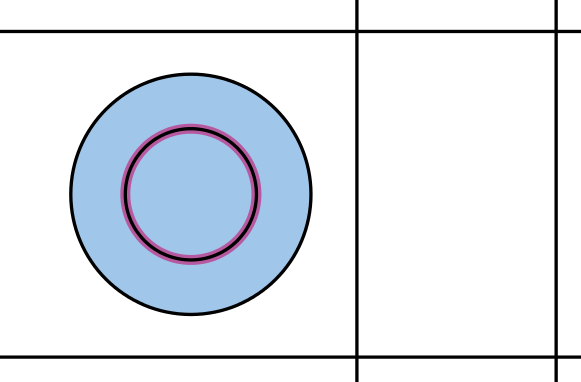
\includegraphics[width=\textwidth]{figures/subd_restrictedFail_c.png}
    %% \caption{xxx} \label{subfig:subd_restrictedFail_c}
  \end{subfigure}%
  \caption[xxx]
          {The restricted algorithm~\ref{alg:subdivisionRestricted} fails when some curves are enclosed inside other faces without intersecting with each other.
          Blue areas show the entailing faces in each case, and the regions that should be substracted from those faces are marked red (what we call super-faces) .}
  \label{fig:subd_restrictedFail}
\end{figure}

To understand the root of this failure, let's construct a multi-directional graph ($\mathit{MDG}$) from all the nodes $\mathcal{N}$ and half-edges $\mathcal{E}$ as demostrated in figure~\ref{fig:subd_mdg}.
The restricted algorithm would work under the assumption that $\mathit{MDG}$ is connected.
This assumption would not hold in the cases of figure~\ref{fig:subd_restrictedFail}.

\begin{figure}%[!ht]
  \centering
  \begin{subfigure}{.32\textwidth}
    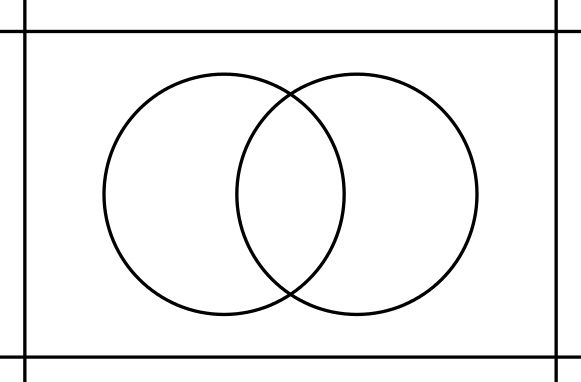
\includegraphics[width=\textwidth]{figures/subd_mdg_a.png}
    \caption{curves} \label{subfig:subd_mdg_a}
  \end{subfigure}%
  ~%
  \begin{subfigure}{.32\textwidth}
    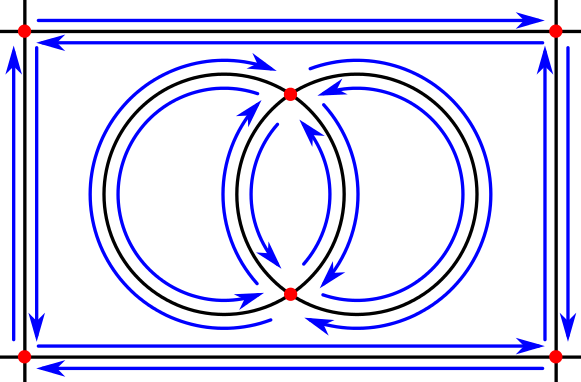
\includegraphics[width=\textwidth]{figures/subd_mdg_b.png}
    \caption{nodes and half-edges} \label{subfig:subd_mdg_b}
  \end{subfigure}%
  ~%
  \begin{subfigure}{.32\textwidth}
    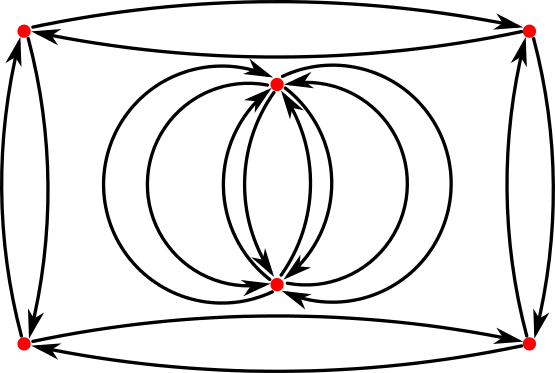
\includegraphics[width=\textwidth]{figures/subd_mdg_c.png}
    \caption{$\mathit{MDG}$} \label{subfig:subd_mdg_c}
  \end{subfigure}%
  \caption[xxx]
          {Construction of a multi-directional graph $\mathit{MDG}$ from nodes and half-edges.
          It is used to identify connected components which result in disconnected partitioning.}
  \label{fig:subd_mdg}
\end{figure}

Sub-graphs (connected components of the $\mathit{MDG}$) being disconnected implies that they are topologically disjoint.
However it does not imply that they are geometrically disjoint.
If there are multiple disconnected sub-graphs, one can be certain that they are either:
\begin{inparaenum}[\itshape i\upshape)]
  \item geometrically disconnected and non-overlapping; or
  \item on subgraph is completely contained in only \emph{one} face of the other subgraph(s).
\end{inparaenum}
Relying on this, we resolve this problem by partitioning each subg-graph of the $\mathit{MDG}$ independently.
And perform a check afterward, to evaluate the relative position of the sub-graphs with respect to each other.
This check relies on the ``membership'' functionality of the subdivision's faces that will be described in section~\ref{subsec:memberNeighbour}.
It involves picking an arbitrary point (node) from each sub-graph and check whether if it is entailed in any other sub-graphs' faces.
If the test implies the overlapping of two sub-graphs, figuratively speaking a hole in the shape of inside sub-graph is punched in the face entailing it\footnote{The face data structure is curated with an attribute of a \emph{hole}.}.
The sub-graphs' outer shape that are colored red in figure~\ref{fig:subd_restrictedFail} are called super-face, and will be described next.
After punching holes, last step to have a whole subdivision would be to append all the faces of each sub-graph to one final list.
This whole process is summerize in the algorithm~\ref{alg:subdivisionComplete} as a complete version of the subdivision algorithm.
%% Assume there are two subgraphs $SG_a$ and $SG_b$ that are geometrically overlapping, but not topologically.
%% That is to say, the subgraphs are plannar and could be drawn on a plane without intersecting each others edges.
%% There is a face in $SG_a$ ($f_i^a \in SG_a$) that all points covered by $SG_b$ would be inside $f_i^a$.
%% To combine these two sub-graphs, we must append all the faces of $SG_b$ to $SG_a$.
%% Then a hole of identified by the ``super-face'' of $SG_b$ must be punched inside $f_i^a$ of $SG_a$.
%% TODO(saesha) Prove this?
%% the important point here is that such a hole in $f_i^a$, does not change other attributes of $SG_a$ and its decomposition.

\begin{algorithm}
  \caption {Subdivision (complete version)}
  \label{alg:subdivisionComplete}
  \begin{algorithmic}
    \STATE INPUT  $\mathcal{C}:\{curves\}$
    \STATE OUTPUT  $\mathcal{F}:\{faces\}$
    \STATE \quad
    \STATE $\mathcal{N}:\{nodes\} = \mathit{intersect} \left( \mathcal{C} \right)$
    \STATE $\mathcal{E}:\{half\text{-}edges\} = \mathit{segment} \left( \mathcal{C}, \mathcal{N} \right)$
    \STATE $\mathit{MDG}= \mathit{multi\_directional\_graph} \left( \mathcal{E}, \mathcal{N} \right)$
    \STATE $\mathcal{SG}:\{sub\_graphs\} = connected\_components(\mathit{MDG})$
    \STATE \quad
    \FORALL {$sub\_graph_i \in \mathcal{SG}$}
    \STATE $ \hat{\mathcal{N}}_i = \{node_j \mid node_j \in sub\_graph_i \} $
    \STATE $ \hat{\mathcal{E}}_i = \{edge_j \mid edge_j \in sub\_graph_i \} $
    \STATE $ \hat{\mathcal{F}}_i= \mathit{partition} \left( \hat{\mathcal{N}}_i, \hat{\mathcal{E}}_i \right)$
    %% \STATE $ subdivision_i = \mathit{Subdivision} \left( \hat{\mathcal{F}} \right) $
    \ENDFOR
    \STATE \quad
    \FORALL {$ sub\_graph_i, sub\_graph_j \in \mathcal{SG}$}
    \IF {$sub\_graph_i \in face_k \mid face_k \text{ belongs } sub\_graph_j$}
    \STATE punch a hole (super-face of $sub\_graph_i$) in $face_k$ of $sub\_graph_j$ 
    \ENDIF
    \ENDFOR
    \STATE \quad
    \STATE $ \mathcal{F} = \displaystyle \bigcup_{i\in I} \hat{\mathcal{F}}_i $, \quad where $I$ is the index set of the $\mathcal{SG}$
  \end{algorithmic}
\end{algorithm}


%%%%%%%%%%%%%%%%%%%%%%%%%%%%%%%%%%%%%%%%
\paragraph{Super-faces}
Incidintally and interesting, one of the useful outcomes of the subdivision algorithm presented in algorithm~\ref{alg:subdivisionComplete} is the detection of what we call a ``super-face''.
For every connected component in the $\mathit{MDG}$, the subdivision algorithm finds one super-face that entails all the other faces of that coonected component of the $\mathit{MDG}$ (see figure~\ref{fig:subd_superface}.)
The algorthim returns the super-face amongst all other faces.
We identify the superface by the size of its surface, which is the biggest face in each subg-graph of the $\mathit{MDG}$.

\begin{figure}%[!ht]
  \centering
  \begin{subfigure}{.32\textwidth}
    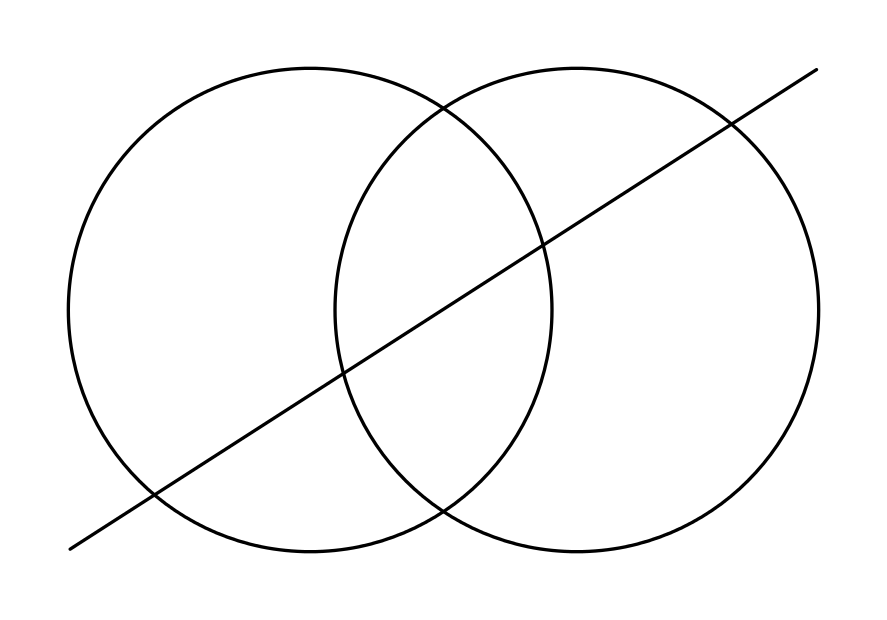
\includegraphics[width=\textwidth]{figures/intro_curves2.png}
    \caption{curves} \label{subfig:subd_superface_a}
  \end{subfigure}%
  ~%
  \begin{subfigure}{.32\textwidth}
    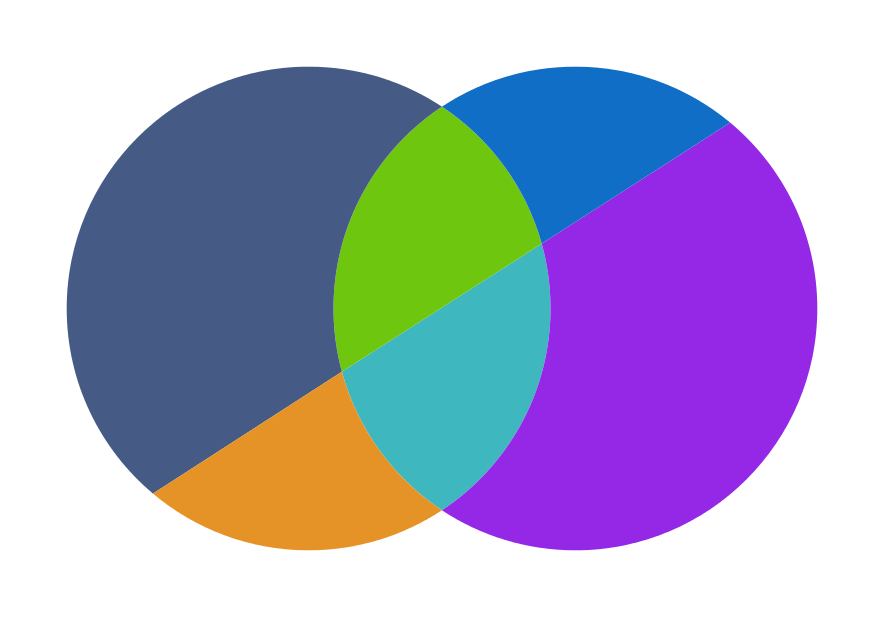
\includegraphics[width=\textwidth]{figures/intro_partitioning2.png}
    \caption{partitioning faces} \label{subfig:subd_superface_b}
  \end{subfigure}%
  ~%
  \begin{subfigure}{.32\textwidth}
    
\includegraphics[width=\textwidth]{figures/subd_superface.png}
    \caption{super-face} \label{subfig:subd_superface_c}
  \end{subfigure}%
  \caption[xxx]
          {Each subdivision process yields a set of partitioning faces, plus a ``super-face'' that covers the whole partitioned area, and represets its outer shape.}
  \label{fig:subd_superface}
\end{figure}

%%%%%%%%%%%%%%%%%%%%%%%%%%%%%%%%%%%%%%%%%%%%%%%%%%%%%%%%%%%%%%%%%%%%%%%%%%%%%%%%
\subsection{Neighbourhood and membership functions} \label{subsec:memberNeighbour}

Neighbourhood functions of a face is handled by the twin concept of half-edges, as described in \cite{de2000computational}.
That is to say, two faces are neighbours if they each have one half-edge with a twin belonging to the other face.

\[
neighbour\left(face_i\right) = \lbrace  face_j \mid \exists e_i, e_i \in face_i, \mathit{twin}(e_i) \in face_j \rbrace
\]

For cases consisting of only straight lines, membership function could be implemented through a set of tests relying on cross products, as described in \cite{de2000computational}.
The tests are to check whether if a point is located on the same side of all the bounding edges of a face.
This would only work if the edge could be represented by a vector.
As can be seen in figure~\ref{fig:intro_crossProdFail}, edges turn to arcs in the presence of circles.
As an alternative we suggest the use of ``point-in-polygon'' method, which is based upon the Jordan Curve theorem \footnote{In fact, as will be described in section~\ref{sec:implementation}, in our implementation each face will be represented by ``path'' class of the matplotlib library. This class, based on b\'ezier curves, provides a method for detecting whether if a given point is located in a closed path. As a consequence the modification of point-in-polygon method is skipped here.}.
Regardless of the method, the membership function behaves as:

\[
member\left(f,p\right) =
\begin{cases}
  1 & \quad \text{if } \left(p \in f\right) \land \left(p \notin hole_i \mid hole_i \in f\right) \\
  0 & \quad \text{otherwise} \\
\end{cases}\\
\]

\begin{figure} %[!ht]
    \centering
    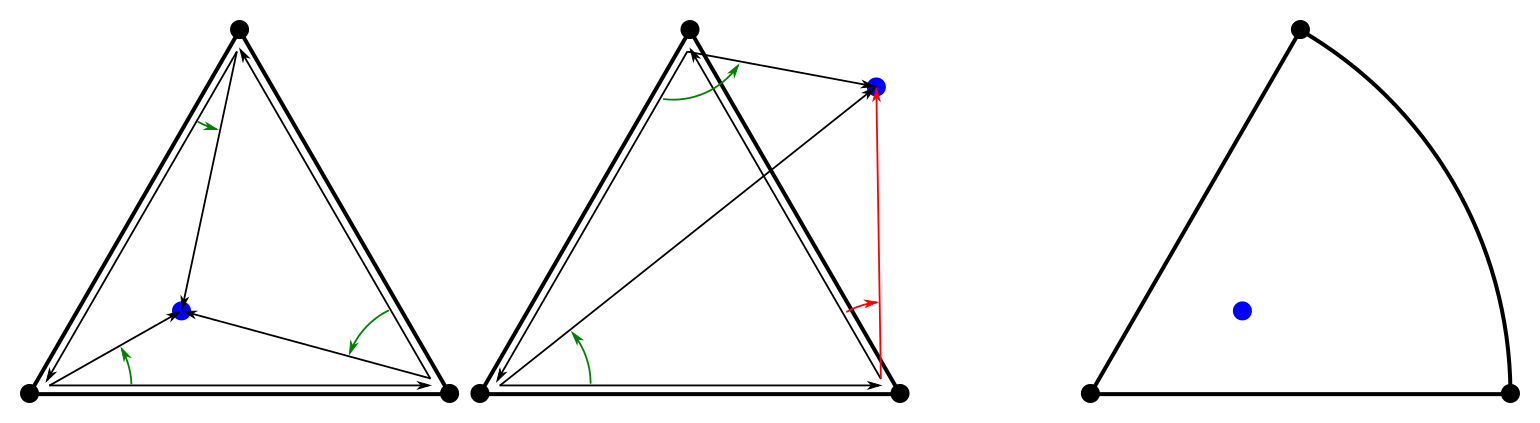
\includegraphics[width=1.\textwidth]{figures/intro_crossProdFail.png}
    \caption{Memebrship function for the case of only straight lines could be based on tests relying on a cross product.
    However, as the edges are no longer vectors in the presence of circles, the conventional membership procedure requires revision.}
    \label{fig:intro_crossProdFail}
\end{figure}

%\section{Implementation} \label{sec:implementation}

This work is accompanied with an implementation of the proposed method in Python \footnote{https://github.com/saeedghsh/subdivision/}.

%% Note:
%% the use of bezier curves for face's path representation is an approximation of the provided curves.
%% This approximation affects both the decomposition (over the area of a face) and accuracy of the point-face localization.
%% Is there any better approach to this approaximation? 

%% Note:
%% faces and holes both belong to face class, but they differ by the direction of their path: 
%% face.path == CCW
%% hole.path == CW

%\section{Discussion} \label{sec:discussion}

%%%%%%%%%%%%%%%%%%%%%%%%%%%%%%%%%%%%%%%%%%%%%%%%%%%%%%%%%%%%%%%%%%%%%%%%%%%%%%%%
\subsection{Degenerate cases}


One degenerate(?) case is due to the ``while-loop'' condition in algorithm~\ref{alg:subdivisionComplete}, where the face identification is terminated as the last half-edge arrives at the starting node.
As can been seen in figure~\ref{fig:disc_specialCase1}, where the hole inside the face is not identified.

\begin{figure} %[!ht]
    \centering
    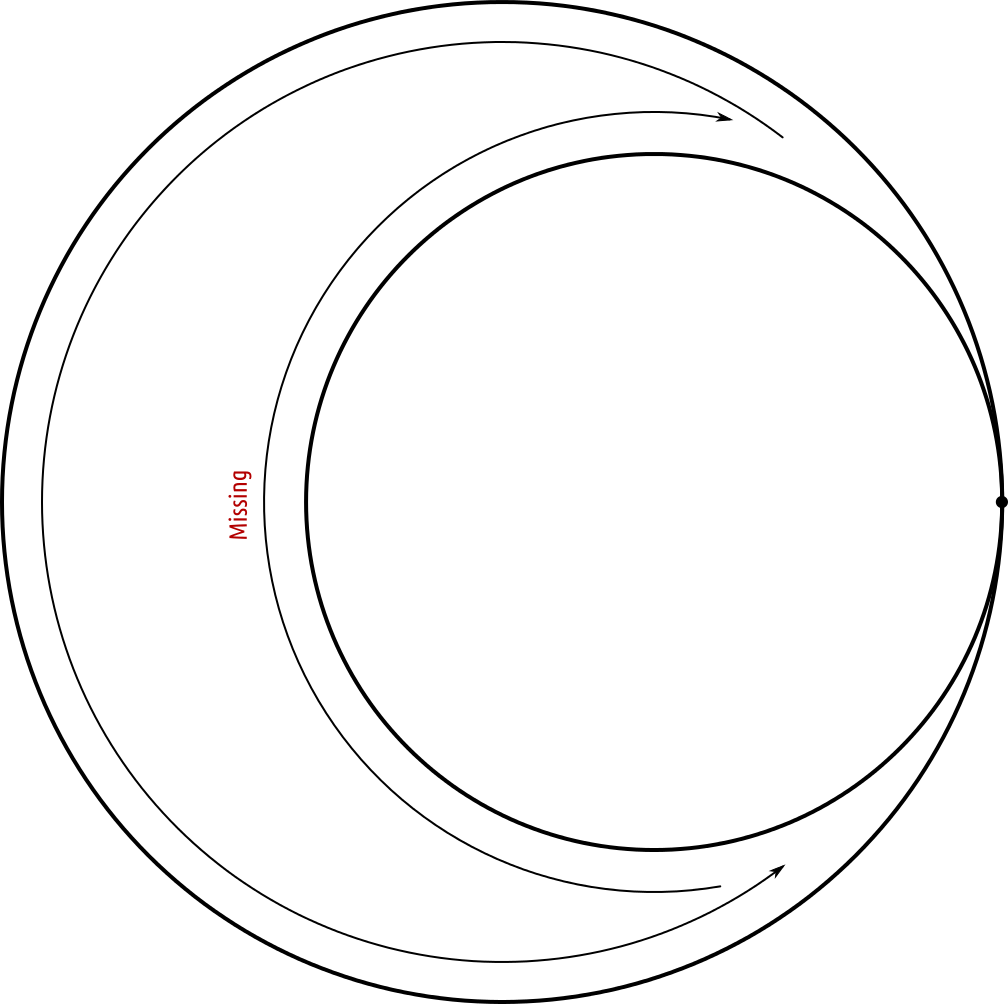
\includegraphics[width=.3\textwidth]{figures/disc_specialCase1.png}
    \caption{xxx}
    \label{fig:disc_specialCase1}
\end{figure}


%%%%%%%%%%%%%%%%%%%%%%%%%%%%%%%%%%%%%%%%%%%%%%%%%%%%%%%%%%%%%%%%%%%%%%%%%%%%%%%%
\subsection{Future work}


%%%%%%%%%%%%%%%%%%%%%%%%%%%%%%%%%%%%%%%%
\subsubsection{Beyond straight lines and circles}

Do we need them? aren't circle and line sufficient for geometric abstraction?

%%%%%%%%%%%%%%%%%%%%%%%%%%%%%%%%%%%%%%%%
\subsubsection{Dynamic subdivision}
%% 1) moving curves: Find ``some conditions'' where as long as they are satisfied, the subdivision maintains the same graph structure, hence the same subdivision.
%% These conditions must be fast to compute (intersection processes is too slow)
%% Could these conditions provide measures for updating the geometry of the subdivision (i.e. attriubutes of nodes and edges).
%% recompute the subdivision
%% 2) adding/removing curves


%%%%%%%%%%%%%%%%%%%%%%%%%%%%%%%%%%%%%%%%
\subsubsection{Face merging, a case of constructive geometry}


\newpage
\begin{appendices}
\section{Univariate representation of the curves} \label{app:alternativeRep}

\paragraph{Line}
The alternative representation of the level-curve of a linear function $f(x,y)=ax+by+c$ could be written as:

\[
\dot{f}(\theta) = (x,y) =
\begin{cases}
  \left( x_l + \theta, y_l \right) & \quad \text{if } s = 0\\
  \left( x_l, y_l + \theta \right) & \quad \text{if } s = \pm \infty\\
  \left( x_l + \dot{a}\theta , y_l + \dot{b}\theta \right) & \quad \text{otherwise} \\
\end{cases}\\
\]

where $(x_l,y_l)$ is an arbitrary (but fixed as a reference) point on the level-curve of the $f(x,y)$, $s$ is the slope of the level-curve of $f(x,y)$, and $\dot{a}, \dot{b}$ are given by:
\[
\dot{a} = \frac{\sqrt{ s^2 + 1}}{s^2 + 1}, \quad \dot{b} = \dot{a}s
\]

The inverse function ($\theta = \dot{f}^{-1}(x,y)$) is given by:
\[
\theta = \dot{f}^{-1}(x,y) =
\begin{cases}
  x & \quad \text{if } s = 0\\
  y & \quad \text{if } s = \pm \infty\\
  \frac{x-x_l}{\dot{a}} & \quad \text{if } \dot{a} \neq 0\\
  \frac{y-y_l}{\dot{b}} & \quad \text{otherwise} \\
\end{cases}\\
\]

While the second derivative of a line is a null vector, the first derivative of a line in this representation would be:
\[
\begin{array}{l}
  \frac{d\dot{f}(\theta)}{d\theta} = \left( \cos(\theta) , \sin(\theta) \right) \text{, where } \theta = \arctan(s)\\
\end{array}
\]



%%%%%%%%%%%%%%%%%%%%%%%%%%%%%%%%%%%%%%%%
\paragraph{Circle}
Similarly, for the level-curve of a conic function $f(x,y)=(x-x_c)^2+(y-y_c)^2-r_c$ (hence the level-curve would be a conic section, in this case a circle) the alternative representation can be written as:

\[
\dot{f}(\theta) = (x,y) = \left( x_c + r_c \cos(\theta), y_c + r_c \sin(\theta) \right)
\]

where $(x_c,y_c)$ is the center of the $f(x,y)$ function, and radius $r_c$ defines the desired level-curve of the $f(x,y)$.\bigskip

The inverse function ($\theta = \dot{f}^{-1}(x,y)$) is given by:

\[
\theta = \dot{f}^{-1}(x,y) = \arctantwo (y - y_c, x - x_c)
\]

The first and second derivatives of a circle in this representation are:
\[
\begin{array}{l}
  \frac{d\dot{f}(\theta)}{d\theta} = \left( -r_c \sin(\theta), r_c \cos(\theta) \right)\\
  \quad\\
  \frac{d^2\dot{f}(\theta)}{d\theta^2} = \left( -r_c \cos(\theta), -r_c \sin(\theta) \right)\\
\end{array}
\]

%%%%%%%%%%%%%%%%%%%%%%%%%%%%%%%%%%%%%%%%
\paragraph{Direction of half-edges and the derivatives}
The half-edges are directed, as the same segment of a curve turns into two half-edges with opposite directions.
Direction of half-edges is very important in the correct calculation of the first derivative vectors.
If a half-edge has a negative direction with respect to the direction of $\theta$, as demonstrated in figure~\ref{fig:appa_derDirection}, its first derivative vectors are rotated $180^o$ degrees to face in the oppposite direction.


\begin{figure}%[!ht]
  \centering
  \begin{subfigure}{.8\textwidth}
    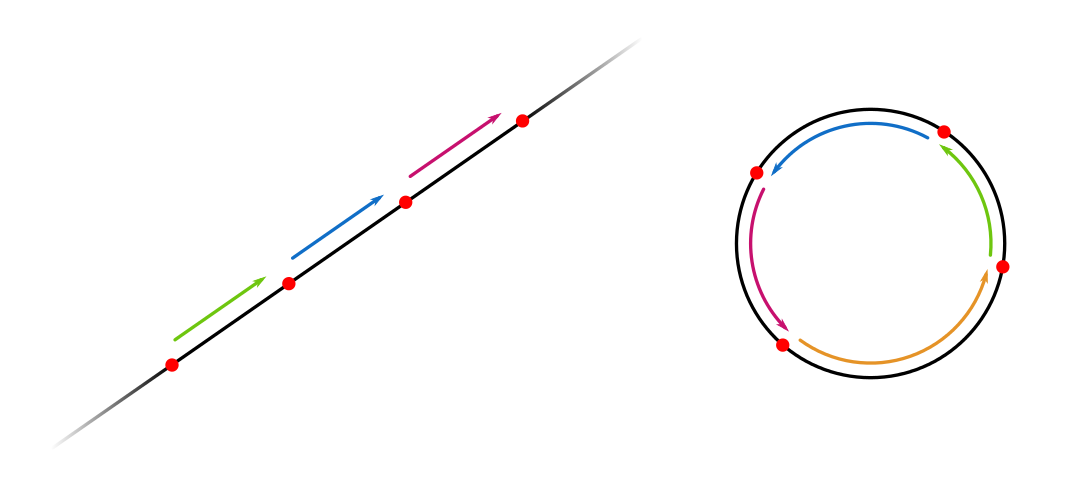
\includegraphics[width=\textwidth]{figures/appa_derDirection_pos.png}
    \caption{half-edges with positive direction} \label{subfig:appa_derDirection_pos}
  \end{subfigure}

  \begin{subfigure}{.8\textwidth}
    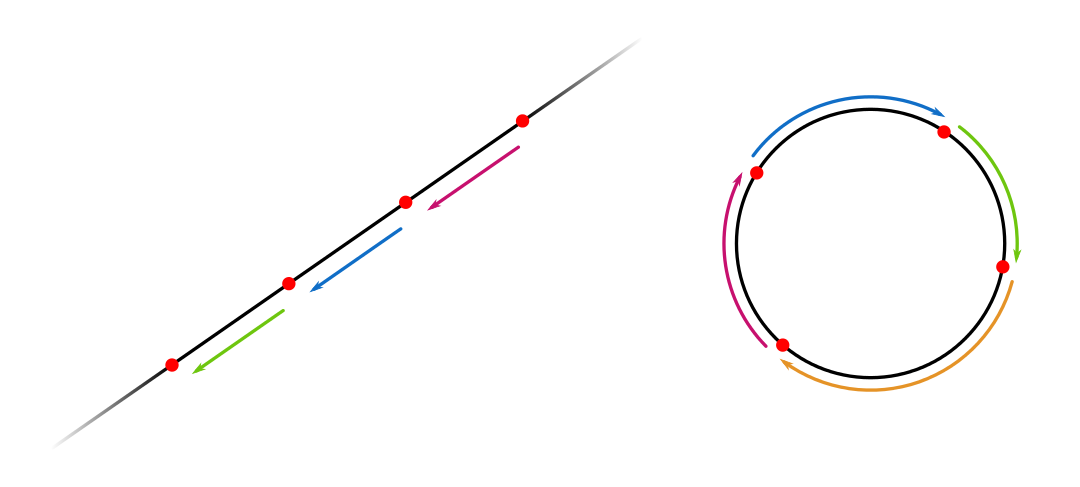
\includegraphics[width=\textwidth]{figures/appa_derDirection_neg.png}
    \caption{half-edges with negative direction} \label{subfig:appa_derDirection_neg}
  \end{subfigure}
  \caption[xxx]
          {Direction of half-edges and its effect on the derivative vectors.}
  \label{fig:appa_derDirection}
\end{figure}




\section{Data Structures} \label{app:datastructure}

%% 1) Doubly Connected Edge List % http://www.ti.inf.ethz.ch/ew/lehre/CG12/lecture/Chapter%205.pdf


\paragraph{Curve}

%% class Circle:
%% DPE
%% IPE
%% firstDerivative
%% secondDerivative

%% class Curve:
%% def __init__(self, curve,
%% self.curve = curve
%% self.ipsIdx = itersectionPointsIdx
%% self.ipsTVal = tValue_at_intersections
%% self.ipsDer1st = at_intersections_derivative_1st
%% self.ipsDer2nd = at_intersections_derivative_2nd

%% assert len(self.ipsIdx) == len(self.ipsTVal)
%% assert len(self.ipsIdx) == len(self.ipsDer1st)
%% assert len(self.ipsIdx) == len(self.ipsDer2nd)


\paragraph{Node}

%% class Node:
%%     def __init__(self, point,
%%                  intersecting_curves_Idx=(),
%%                  intersecting_curves_Tval=()):
        
%%         self.point = point
%%         self.curveIdx = intersecting_curves_Idx
%%         self.curveTval = intersecting_curves_Tval


\paragraph{Half-Edge}

%% class HalfEdge:
%%     def __init__ (self,
%%                   selfIdx, twinIdx,
%%                   cIdx, side,
%%                   sIdx, sTVal, s1stDer, s2ndDer,
%%                   eIdx, eTVal, e1stDer, e2ndDer):

%%         self.selfIdx = selfIdx   # (sIdx, eIdx, pIdx)
%%         self.twinIdx = twinIdx   # twin half edge's index

%%         # half edge Curve's attributes:
%%         self.cIdx = cIdx         # Index of the curve creating the edge
%%         self.side = side         # defines the direction of t-value (in: t2>t1, out: t1>t2)
        
%%         # half edge attributes:
%%         self.sIdx = sIdx         # starting node's index        
%%         self.sTVal = sTVal
%%         self.s1stDer = s1stDer
%%         self.s2ndDer = s2ndDer

%%         self.eIdx = eIdx         # ending node's index
%%         self.eTVal = eTVal
%%         self.e1stDer = e1stDer
%%         self.e2ndDer = e2ndDer

\paragraph{Face}
%% (also, holes and patches)

%% class Face:
%%     def __init__(self, halfEdgeList, path):
%%         ''' '''
%%         self.halfEdges = halfEdgeList
%%         self.path = path
%%         self.holes = () # list of faces

%%     def get_area(self, considerHoles=True):
%%         '''
%%         Be aware that path.to_polygons() is an approximation of the face,
%%         if it contains curves, consequently the area would be approximated

%%         Green's theorem could provide an accurate measure of the area
%%         '''
%%         polygon = self.path.to_polygons()
%%         assert len(polygon) == 1
%%         x = polygon[0][:,0]
%%         y = polygon[0][:,1]
%%         PolyArea = 0.5*np.abs(np.dot(x,np.roll(y,1))-np.dot(y,np.roll(x,1)))
        
%%         holesArea = 0
%%         if considerHoles:
%%             for hole in self.holes:
%%                 polygon = hole.path.to_polygons()
%%                 assert len(polygon) == 1
%%                 x = polygon[0][:,0]
%%                 y = polygon[0][:,1]
%%                 holesArea += 0.5*np.abs(np.dot(x,np.roll(y,1))-np.dot(y,np.roll(x,1)))

%%         return PolyArea - holesArea

%%     def is_point_inside(self, point):
%%         ''' '''
%%         if self.path.contains_point( (point.x,point.y) ):
%%             for hole in self.holes:
%%                 if hole.path.contains_point( (point.x,point.y) ):
%%                     return False
%%             return True        
%%         return False

%%     def punch_hole(self, holeFace):
%%         ''' '''
%%         self.holes += (holeFace,)


%%     def get_punched_path(self):
%%         '''
%%         this is only useful for plotting
%%         the "path.contain_point()" doesn't work with holePunched pathes anyway

%%         no need to invert holes' trajectory,
%%         as they are supposedly superfaces, which means they have cw trajectory
%%         '''
%%         verts = self.path.vertices
%%         codes = self.path.codes

%%         for hole in self.holes:
%%             verts = np.append( verts, hole.path.vertices, axis=0)
%%             codes = np.append( codes, hole.path.codes)

%%         return mpath.Path(verts, codes)


        
\paragraph{Decomposition}
%% class Decomposition:
%%     def __init__ (self, graph, faces, superFaceIdx=None):
        
%%         self.graph = graph

%%         if superFaceIdx is not None:
%%             f = list(faces)
%%             self.superFace = f.pop(superFaceIdx)
%%             self.faces = tuple(f)
%%         else:
%%             self.superFace = None
%%             self.faces = faces

%%     def find_face(self, point):
%%         for idx,face in enumerate(self.faces):
%%             if face.is_point_inside(point):
%%                 return idx
%%         return None

%%     def find_neighbours(self, faceIdx):
%%         return []
        
%%     def get_extents(self):
%%         bboxes = [face.path.get_extents() for face in self.faces]
%%         return matplotlib.transforms.BboxBase.union(bboxes)


\paragraph{Subdivision} \quad

\end{appendices}

\bibliographystyle{plain}
\bibliography{mybib.bib}

\end{document}